\part{Socio-histoire d'un musée à part}

%%%%%%%%%%%%%%%%%%%%%%%%%%%%%%%%%%%%%%%%%%%%%%%%%%%%%%%%%%%%%%%%%%%%%%%%%%%%%%%%%%%%
%%%%%%%%%%%%%%%%%%%%%%%%%%%%%%%%%%%%%%%%%%%%%%%%%%%%%%%%%%%%%%%%%%%%%%%%%%%%%%%%%%%%
%%%%%%%%%%%%%%%%%%%%%%%%%%%%%%%%%%%%%%CHAPITRE%%%%%%%%%%%%%%%%%%%%%%%%%%%%%%%%%%%%%%
%%%%%%%%%%%%%%%%%%%%%%%%%%%%%%%%%%%%%%%%%%%%%%%%%%%%%%%%%%%%%%%%%%%%%%%%%%%%%%%%%%%%
%%%%%%%%%%%%%%%%%%%%%%%%%%%%%%%%%%%%%%%%%%%%%%%%%%%%%%%%%%%%%%%%%%%%%%%%%%%%%%%%%%%%

\chapter{Une bibliothèque, un musée et une association unique en France, au service du « Beau dans l’Utile »}

\section{Le \textsc{XIX}\textsuperscript{e}~siècle et les arts décoratifs}

Au cours de ce siècle d'intense industrialisation, la position de l'artiste à l'intérieur de la société évolue. La dimension holistique du \enquote{savoir technique de l'artisan est niée et fragmentée par la division du travail, il se transforme en exécuteur passif d'une œuvre dont la conception ne lui appartient plus}\footnote{\cite{froissart_union_1990}. p. 1.}. Le statut de l’œuvre change aussi, elle perd sa connotation artistique originale du fait de sa reproductibilité technique, et se retrouve dépourvue de son \enquote{aura}\footnote{\cite{benjamin_walter_oeuvre_2013}}. À partir des années 1830, et au fil des expositions universelles, les arts industriels s'imposent petit à petit mais ne gagnent jamais la dignité réservée aux Beaux-Arts. On les considère comme des objets \enquote{produit à bon marché et en série, [...] forcément laids}\footnote{\cite{froissart_union_1990}. p. 11.}. Il faut attendre 1861 pour voir en France une première exposition dédiée aux arts industriels. Elle ne voit le jour qu'\enquote{avec des moyens limités et grâce à l'initiative privée}\footnote{\cite{froissart_union_1990}. p. 17.}. 

Les initiateurs de cette exposition sont ceux qui sont aussi derrière la fondation d'une association dédiée aux arts industriels quelques années plus tard. Ils ont pour ambition l’anoblissement de ces arts et leur pleine inscription dans le paysage artistique de leur époque. Cette entreprise de légitimation est la mieux représentée par la position d'un homme de lettres et journaliste, Théodore Labourieu, qui joue un rôle majeur en faveur des arts décoratifs en ce milieu du \textsc{xix}\textsuperscript{e}~siècle. Il \enquote{engage une vraie bataille contre tous ceux qui veulent reléguer les arts appliqués dans le domaine méprisé de l'industrie et du commerce, indignes donc de rechercher le vrai beau \textit{idéal}}\footnote{\cite{froissart_union_1990}. p. 33.}. Il critique le \textquotedblleft grand Art\textquotedblright{} qu'il appelle \textquotedblleft abstrait\textquotedblright{}, et à qui il reproche d'appartenir à la sphère de l'idéal et non de la réalité concrète. Il va plus loin en disant qu'\enquote{il n'est pas l'expression de son époque ; [et que] seul l'art qui contribue directement à satisfaire les besoins pratiques de l'homme est capable d'exprimer son siècle, le siècle du \textquotedblleft Travail\textquotedblright{}}\footnote{\cite{labourieu_art_1857}. p. 261.}.
Son ambition est de rapprocher l'art du public, et il voit dans l'art uni au travail, dans le syncrétisme entre artiste et ouvrier, la voie que doit emprunter l'art nouveau dessiné par ce siècle industrieux. C'est animé d'une foi dans le travail comme moyen de progrès, empreinte des idées des socialismes contemporains et du saint-simonisme que Labourieu théorise cette mise à la portée de l'art pour chacun\footnote{\cite{froissart_union_1990}. p. 33.}. 

\subsection{Fondation et historique de l'association}

L'histoire de l'entité qui regroupe deux musées, une école, une bibliothèque et une association sous le même sigle "MAD" de nos jours, remonte à cette deuxième moitié de \textsc{xix}\textsuperscript{e}~siècle et prend racine dans deux mémoires et un placet remis à Charles Louis Napoléon Bonaparte alors président de la Deuxième République, peu de temps avant la proclamation de l'Empire. Ces documents lui sont remis le 25 novembre 1852\footnote{\cite{noauthor_origines_nodate}. p. 3.} à Saint-Cloud de la part du "Comité central des artistes et des artistes industriels" qui représente 126 artistes, dessinateurs industriels, architectes, sculpteurs, graveurs, ornemanistes et joailliers. Le but de ces doléances est \enquote{de demander à l'État d'instaurer un musée des beaux-arts industriels, une école centrale des beaux-arts appliqués à l'industrie et des expositions spéciales des œuvres des artistes industriels}\footnote{\cite{noauthor_origines_nodate}. p. 3.}. 

Ces doléances restent lettre morte, et c'est Théodore Labourieu qui, en 1855, reprend le propos de ces mémoires et décide d'en soutenir les visées par la création de la revue \textit{L'art au \textsc{xix}\textsuperscript{e}~siècle}\footnote{\cite{froissart_union_1990}. p. 21.}. C'est dans cette revue que sont publiés les premiers statuts de l'association du nom de Société pour le Progrès des Arts Industriels en 1858, présidé par M. Mirault, à la suite de la présentation d'un projet d'école et de musée au Conservatoire des Arts et Métiers le 14 juillet 1856\footnote{\cite{froissart_union_1990}. p. 23.}. 
À l'origine le musée ne devait \enquote{qu'être complémentaire à l'école, [...] pour que les ouvriers puissent avoir le temps de visiter ses collections de modèles}\footnote{\cite{froissart_union_1990}. p. 36.}. L'idée principale est la création d'une école d'arts appliqués au sein du Conservatoire des Arts et Métiers, et les initiateurs savent que le musée sera le résultat d'une démarche plus longue.

Après plusieurs années de tentatives d'expositions infructueuses c'est Édouard Guichard qui obtient, avec le concours du baron Taylor, une première exposition fin 1861 au Palais de l'Industrie. 
\vspace{1em}

\noindent
\hspace*{1cm}
\begin{minipage}{\dimexpr\linewidth-2cm}
\fontsize{10}{12}\selectfont
Le but de l'initiative est de pousser les artistes à une émulation féconde, de mieux définir leurs place à l'intérieur de domaines éloignés comme ceux de l'industrie et de l'art [et peut-être d'amener] l'art industriel à une fonction vulgarisatrice de l'idée du \textit{beau}, \textit{vrai}, et \textit{bien}                                                        \footnotemark{}
\end{minipage}

\vspace{1em}

\footnotetext{insère la ref bibliographique}

\footnotetext{\cite{froissart_union_1990} p. 40.}

Après l'exposition de 1863, la Société pour le Progrès des Arts Industriels entre en crise profonde et se dissout, ce qui amène la fondation en 1864 de l'Union centrale des Beaux-Arts appliqués à l'Industrie dont le siège est établi au 3 places des Vosges, au plus près des ouvriers du Marais. Dans ses statuts, son but est \enquote{d'entretenir en France la culture des arts qui poursuivent la réalisation du beau dans l'utile ; de recevoir, d'augmenter et de tenir à la disposition des travailleurs, les collections d'objets d'arts anciens [sic] et modernes, et la bibliothèque}\footnote{\cite{noauthor__1864}}. 

Sont aussi établies des expositions de collections particulières. Les premières pièces de ce musée nouveau se composent principalement des objets offerts à l'Union à la suite de l'exposition de l'année 1863 au Palais de l'Industrie. On y trouve aussi des \enquote{objets de haute curiosité, libéralement prêtés par des collectionneurs qui désirent concourir à cette œuvre}\footnote{\cite{noauthor_origines_nodate}. p. 8.}. Il s'agit de faïences, d'étoffes vénitiennes, de vêtements asiatiques, de tapisseries des Gobelins, etc,. Ces objets exposés sont renouvelés tous les trois mois pour offrir aux fabricants et ouvriers de nouveaux sujets d'études.

\subsection{La bibliothèque}

Avant l'ouverture de la Bibliothèque de l'Union Centrale des Beaux-Arts appliqués à l'industrie, et de la Bibliothèque Nationale des Beaux-Arts la même année, il n'existait pas, à Paris, de bibliothèque spéciale d'art\footnote{\cite{noauthor__1955}. p. 1.}. À l'origine la bibliothèque est le \enquote{premier embryon} de l'Union\footnote{\cite{noauthor__1991}. p. 2.}. Elle est ouverte au sein du siège social place des Vosges, là où le musée s'ouvre aussi dans un premier temps, avant d'être transféré au Pavillon de Flore, dans le Louvre, et de rejoindre enfin le Palais de l'Industrie. Cette bibliothèque est ouverte à tous\wokisme tes et gratuite, les lecteurs\wokisme trices doivent simplement remplir un bulletin avec leur nom, profession et adresse pour accéder aux collections. Yvonne Brunhammer souligne dans son ouvrage de 1992, à propos de la Bibliothèque de l'UCAD, qu'elle \enquote{suscite les commentaires les plus élogieux. Les journalistes y voient, à juste titre, la justification de l'action de l'Union centrale en faveur de l'art industriel}\footnote{\cite{brunhammer_beau_1992}. p. 22.}. En effet, c'est un lieu \enquote{unique en son genre, en ce que les lecteurs sont autorisés à copier mais aussi à calquer les modèles}\footnote{\cite{noauthor__1874}.}. À ses débuts la bibliothèque n'a pas encore un fonds important, environ 4000 volumes de dessins, des échantillons d'étoffes, des maquettes pour soieries, des impressions sur mousseline et des papiers peints. Cependant, à la faveur de mécénats et de l'implication de personnalités comme Jules Maciet, les collections s'enrichissent considérablement au cours du \textsc{xix}\textsuperscript{e}~siècle, notamment avec la constitution des albums Maciet où sont regroupés par thèmes les reproductions d’œuvres et d'iconographies glanées au fil des livres, catalogues d'expositions et de ventes collectées et découpées à même les ouvrages pour les assembler.

La bibliothèque déménage au tournant du \textsc{xx}\textsuperscript{e}~siècle dans les locaux du Pavillon de Marsan et constitue une collection importante, témoignage de l'histoire de la technique au service du goût et de la mode au cours des derniers siècles. On y trouve, au milieu du \textsc{xx}\textsuperscript{e}~siècle plus de 75 000 volumes de livres, de périodiques, de catalogues de ventes ou d'expositions. Il y a aussi 700 albums de dessins et d'échantillons de tissus, soieries, rubans, dentelles et papiers peints. Environ 60 000 dessins originaux, que ce soit de dessins d'architectures, d'ornements, de jardins, de céramiques, d'orfèvreries, de mobilier. \hfill \pagebreak

\subsection{Le musée}

Le musée de son côté, \enquote{semble avoir été fragile et temporaire} dans les premiers temps\footnote{\cite{gady_dessin_2020}. p. 12.}. Dans le carton d'invitation pour l'inauguration au 20 septembre 1864 est indiqué une ouverture jusqu'au 30 novembre seulement\footnote{\cite{noauthor__1864-1}}. \enquote{Le musée s'étendait sur deux salles qui faisaient pendant à celles de la bibliothèque, et dont la deuxième servait aussi de salle de conférences}\footnote{\cite{gady_dessin_2020}. p. 12.}. Pour remédier à la maigre dotation du musée, qui était essentiellement fondée sur des prêts, une souscription est lancée en 1876 pour étendre les collections\footnote{\cite{noauthor__1876}}. En 1877, à la veille de l'Exposition Universelle de 1878, la Société du musée des arts décoratifs (Smad) est fondée par des grands collectionneurs, aristocrates, banquiers et industriels. Cette action concertée, avec le concours de l'État, permet au musée de se déplacer provisoirement au Pavillon de Flore, où l'exposition de chefs-d’œuvres prêtés par des particuliers rencontre un succès retentissant. Néanmoins, après une année, le musée est mis à la porte du Pavillon de Flore au profit de la préfecture de la Seine et doit se déplacer dans les locaux peu appropriés du Palais de l'Industrie\footnote{\cite{froissart_union_1990}. p. 124.}.

Au moment de ces déménagements et de ce rapprochement avec la Smad, le fonctionnement de l'Union est amendé, notamment en ce qui concerne la constitution de son patrimoine financier. Après 1874, la capital de l'Union n'est plus constitué par les \enquote{souscriptions, dons, droits d'entrée dans les galerie d'expositions, mais représenté essentiellement par des actions, émises au nombre de 4000}\footnote{\cite{froissart_union_1990}. p. 92.}. La Société du musée des arts décoratifs est \enquote{peut-être [aussi] née de l'impossibilité juridique pour l'Union [d'alors] d'encaisser les fruits de la souscription pour l'extension du musée} du fait de ce changement de statut\footnote{\cite{noauthor__1876}\enquote{\textit{En effet, dans notre organisation actuelle, nous ne sommes pas autorisés à accepter des fonds affectés à une destination qui exigerait une gestion à part, entraînant la société hors des limites que la loi nous prescrit de ne pas franchir}} cité dans \cite{gady_dessin_2020}. p. 19.}. 

\section{Un statut hybride, des collections protéiformes}

D'abord perçue comme concurrentes, \enquote{l'Union centrale et la Société du musée des Arts décoratifs sont condamnées à s'entendre, malgré leur divergences d'origine et d'opinion : les fondateurs de l'Union centrale appartiennent au monde des industries d'arts, les initiateurs de la Société du musée sont des leaders politiques et mondains}\footnote{\cite{brunhammer_beau_1992}. p. 35.}. Après leur fusion sous le nom d'Union Centrale des Arts Décoratifs en 1880, ils s'unissent dans la recherche d'un lieu pour le musée et la bibliothèque. L'entité issue de cette fusion, fruit de deux initiatives privées, est \enquote{adoubée} par l'État avec le décret qui la reconnaît d'utilité publique le 15 mai 1882. À côté de cette reconnaissance, dès les débuts de la Smad, on réflechit à la forme que prendrait une convention avec l'État afin de pérenniser le projet de musée. 

\subsection{Les donateurs et bienfaiteurs}

Le souffle qu'apporte la création de l'UCAD, et la réunion de ces volontés convergentes, amène aux premières campagnes de dons qui constitueront le noyau des collections. On peut citer Alphonse Wyatt Thibaudeau, marchand londonien, Philippe Chennevières, président par intérim de l'UCAD, ou bien Jules Maciet qui offrent la même année un corpus de dessins de maîtres et d'ornements aux collections de la nouvelle Union. Du côté du musée comme de la bibliothèque les deux décennies de cette fin \textsc{xix}\textsuperscript{e}~siècle sont marquées par un accroissement des collections. À la bibliothèque, c'est notamment son conservateur, par l'entremise de la \textit{Revue des arts décoratifs}, qui lance des appels aux dons de gravures et de photographies afin de constituer une collection encyclopédique ou iconographique. Cependant, le musée aussi collecte dessins et gravures, et malgré le fait que \enquote{tous les textes [de l'époque] insistent sur la nécessaire union de la bibliothèque et du musée, les deux entités géraient séparément leurs achats et leurs dons}\footnote{\cite{gady_dessin_2020}. p. 14.}. 

Un principe de séparation semblait exister, dans le cas par exemple où un don était adressé à l'UCAD, sans précision supplémentaire de l'institution à laquelle le don était destiné. On attribuait les dessins de maîtres au musée et les recueils de fonds complets, ou les dessins isolés jugés de moindre qualité à la bibliothèque. Cependant, ce n'était pas un principe absolu et \enquote{des glissements ponctuels d'une entité vers l'autre apparaissait fréquemment sur les registres, parfois à plusieurs reprises}\footnote{\cite{gady_dessin_2020}. p. 14}. Ces aller-retours, conjugués avec les politiques d'acquisition respectives de deux institutions de l'Union et la générosité des donateurs, créent les conditions pour donner naissance \enquote{à un trésor partiellement inexploré} du fait aussi des faibles moyens de cette institution associative\footnote{\cite{gady_dessin_2020}. p. 10.}. 

La structure associative de cette institution a toujours demandé à ses membres un investissement personnel important, mais aussi un désintéressement matériel marqué. C'est aussi cela qui fait \enquote{l'originalité de cette institution privée entièrement dévouée au public, dans un panorama français alors si marqué par le rôle de l'État}\footnote{\cite{gady_dessin_2020}. p. 15.}. En effet, outre la gratuité de l'accès à la bibliothèque, le musée aussi est ouvert gratuitement au public. C'est notamment cette liberté et cette créativité qui ont permis d'élargir le cercle de ses bienfaiteurs. Souvent les descendants d'artistes exposés qui ont profité de cette libéralité, ou bien les veuves d'artistes offraient dessins et archives personnelles à l'UCAD en signe de reconnaissance et pour prendre part à ce projet commun. 

\subsection{Le rôle de l'État central}

Comme nous l'avons vu, la genèse du projet de l'UCAD prend racine dans une doléance formulée à l'État central, que celui-ci ignore. C'est cet échec fondateur qui préside finalement à la forme et à la structuration si singulière de l'institution qu'est aujourd'hui le MAD, héritière de ces enjeux et de ces négociations constantes avec le pouvoir. C'est réellement avec la problématique de l'installation du musée dans un endroit plus adapté à la conservation des collections que le Palais de l'Industrie, que commencent les tractations soutenues avec l'État. Il est d'abord question d'une installation dans les anciens locaux de la Cour des Comptes et du Conseil d'État (incendiés pendant la Commune en 1871) sur le Quai d'Orsay (qui deviendra le Musée d'Orsay), et un projet de convention en ce sens est soumis aux deux parties en février 1885\footnote{\cite{froissart_union_1990}. p. 143.}. C'est finalement la destruction en 1896 du Palais de l'Industrie qui précipite les choses. Cette année-là, les collections du musée sont transférées au Pavillon de Marsan dont la concession avait été promise par l'État. 

L'année suivante est signée la première Convention liant l'UCAD à l'État. Elle ne stipule pas de renouvellement possible, et est résiliable à tout moment par l'État. Elle concède pour 15 années les locaux du Pavillon de Marsan à l'UCAD en échange de la prise en charge par l'Union de travaux d'aménagement, de la prise en charge de son entretien et de la soumission aux impôts liés au bâtiment. La gratuité d'accès pour le public est partiellement révoquée. Au terme de ces 15 ans, l'État reprend les locaux aménagés et \enquote{les collections feront retour à l'État sous le nom de Musée National des Arts Décoratifs, l'État entrant de plein droit et sans indemnité dans la propriété pleine et entière [...] des collections}\footnote{\cite{noauthor__1970}. p. 3.}. C'est donc avec l'assurance d'avoir un endroit pour unifier les deux organes principaux de l'UCAD, sa bibliothèque et son musée, que s'achève ce \textsc{xix}\textsuperscript{e}~siècle et que commencent huit années de travaux pour le Pavillon de Marsan.

\begin{figure}
    \centering
    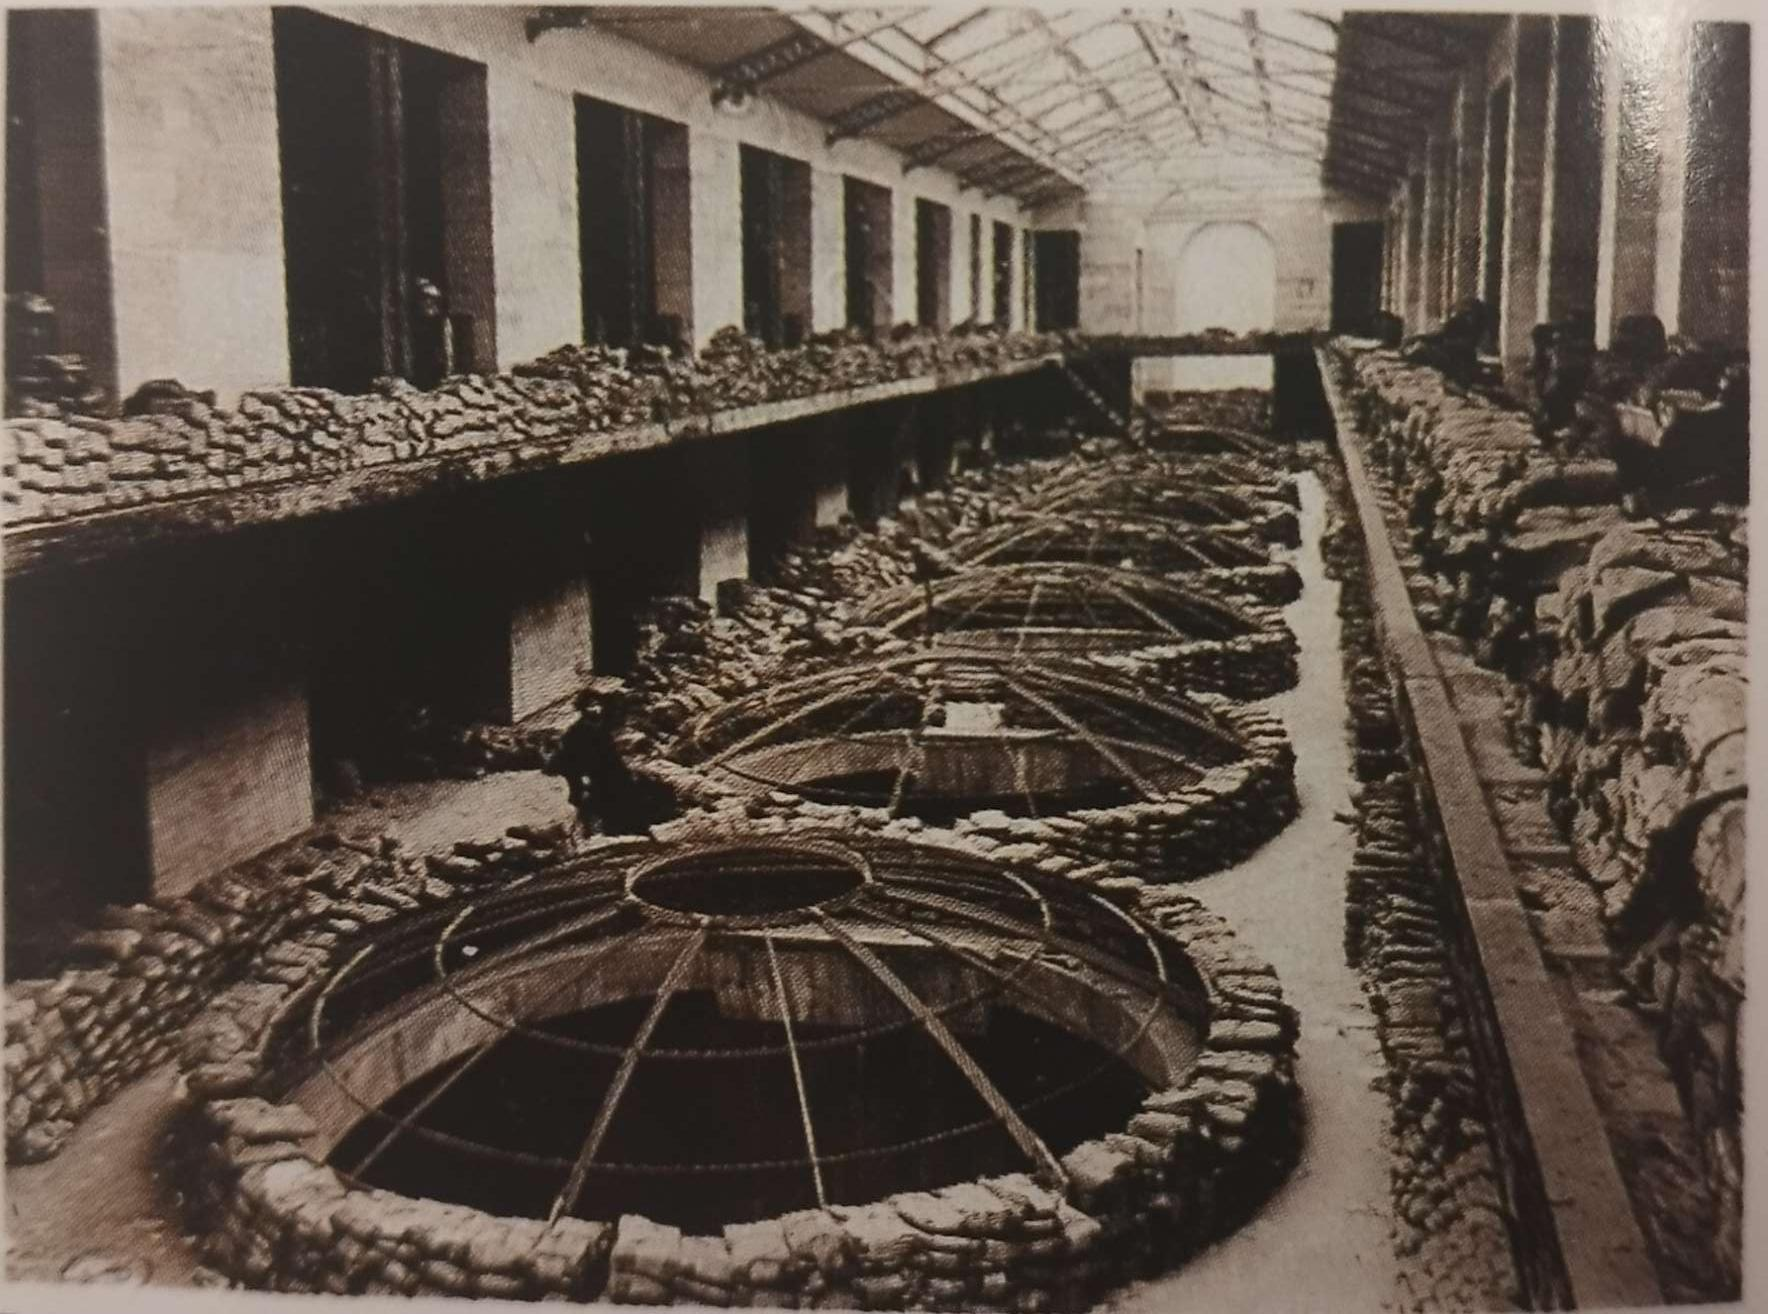
\includegraphics[width=0.75\linewidth]{Illustrations/1.jpg}
    \caption{Photo d'archive de la nef encombrée par les dossiers de la Cour des Comptes autour de 1900}
    \label{fig:placeholder}
\end{figure}

%%%%%%%%%%%%%%%%%%%%%%%%%%%%%%%%%%%%%%%%%%%%%%%%%%%%%%%%%%%%%%%%%%%%%%%%%%%%%%%%%%%%
%%%%%%%%%%%%%%%%%%%%%%%%%%%%%%%%%%%%%%%%%%%%%%%%%%%%%%%%%%%%%%%%%%%%%%%%%%%%%%%%%%%%
%%%%%%%%%%%%%%%%%%%%%%%%%%%%%%%%%%%%%%CHAPITRE%%%%%%%%%%%%%%%%%%%%%%%%%%%%%%%%%%%%%%
%%%%%%%%%%%%%%%%%%%%%%%%%%%%%%%%%%%%%%%%%%%%%%%%%%%%%%%%%%%%%%%%%%%%%%%%%%%%%%%%%%%%
%%%%%%%%%%%%%%%%%%%%%%%%%%%%%%%%%%%%%%%%%%%%%%%%%%%%%%%%%%%%%%%%%%%%%%%%%%%%%%%%%%%%

\chapter{Le XXe siècle, le Pavillon de Marsan et la gouvernance}

La nouvelle période qui s'ouvre pour l'UCAD avec l'accession aux locaux du Pavillon de Marsan et de l'aile de Rohan verra l'Union, le musée et sa bibliothèque se transformer. Leurs collections vont s'étendre et se patrimonialiser, et les publics vont progressivement changer à la faveur de cette patrimonialisation. Les artisans et dessinateurs seront peu à peu remplacés par les étudiants et amateurs d'arts. C'est aussi la période pendant laquelle les rapports entre l'État et l'UCAD vont se préciser et s'ancrer, au gré des luttes d'influences du pouvoir central et des manœuvres qu'entreprend l'association pour conserver son indépendance. Cette période verra pas moins de 5 conventions signées entre l'État et l'UCAD pour la concession du Pavillon de Marsan, avec par moments des changements structurels importants. Et \enquote{de convention en convention perdure ce statut si surprenant d'une collection nationale abritée dans des bâtiments de l'État, gérée grâce à une importante subvention publique, mais augmentée, restaurée, exposée et diffusée aux frais d'une association}\footnote{\cite{gady_dessin_2020}. p. 17.}.

\section{1905 : date fondatrice pour le musée et l'association}

Le 29 mai 1905, l'inauguration officielle du musée a lieu en présence du Président de la République Emile Loubet. Les sommes engagées pour les travaux de restauration par l'UCAD s'élèvent à 8 millions de francs. En réalité, une ouverture partielle depuis 1902 a permis au musée d'organiser ses premières expositions, mais son installation pleine et entière dans les locaux est retardée par la présence de centaines de milliers de liasses d'archives de la Cour des Comptes qui encombrent le pavillon de Marsan. 

\subsection{L'enrichissement des collections, méthodes d'acquisitions et donations}

Le statut loi 1901 de l'UCAD et sa reconnaissance d'utilité publique lui permettent de recevoir en plus des dons manuels, les legs et donations pour alimenter ses collections. Souvent les membres du Conseil d'administration sont aussi des donateurs à l'image de Jules Maciet, Paul Gasnault ou plus tard David David-Weill. Vient ensuite un legs d'importance pour les collections du musée, le legs Peyre. Puis, de façon générale, l'Union adopte une posture active dans l'achat d’œuvres pour alimenter ses collections. 

L'institution a cela de particulier qu'elle est aussi musée de séries d'objets et d'ensembles. Elle acquiert aussi des pièces uniques qui représentent leur temps ou une maîtrise particulière, mais le \textsc{xx}\textsuperscript{e}~siècle verra nombreuses manufactures, entreprises, ateliers, bijouteries donner en bloc des créations. Sans compter les ensembles constitués par les particuliers et collectionneurs qui cèdent leurs collections dans leurs testaments. C'est de cette manière que le Musée Camondo voit le jour le 21 décembre 1936 sous l'égide de l'UCAD. Le Comte Moïse de Camondo, en l'absence d'héritier, lègue un hôtel particulier, ses collections et des rentes suffisantes pour que soit édifié le Musée Nissim de Camondo, du nom de son fils défunt. 

Il faut aussi noter la procédure à laquelle l'association doit se soumettre afin de pouvoir accepter les dons et legs.

\vspace{1em}

\noindent
\hspace*{1cm}
\begin{minipage}{\dimexpr\linewidth-2cm}
\fontsize{10}{12}\selectfont
Les donations et les legs sont des types d’acquisitions pour lesquelles les dispositions doivent être authentifiées par des actes écrits. La donation est la transmission d’un bien à titre gratuit ; elle doit être passée devant notaire et acceptée par le bénéficiaire, à la différence du don, transmission moins procédurière qui n’engendre pas obligatoirement d’écrits. \footnotemark{}                                                     
\end{minipage}

\vspace{1em}

\footnotetext{\cite{siguret_ir_2001}. p. 29.}

 Ce point souligne par ailleurs l'un des problèmes principaux de nombreuses œuvres qui font partie des collections du musée : les artistes ou les manufactures qui donnent quantité d'ouvrages avec une simple note manuscrite indiquant par exemple \enquote{La manufacture Leroy donne un lot de papier peint.} 

Cela génère deux problèmes majeurs pour les conservateurs\wokisme trices, d'abord le manque de description du fonds, ce qui rend difficile le travail scientifique, puis le problème des droits qui surgit souvent dans ce genre de dons, où les descendant\wokisme e \wokisme s réclament des compensations dans le cas où les droits de publications ou de reproductions n'ont pas été spécifiquement accordés à l'institution. 
\vspace{1em}

\noindent
\hspace*{1cm}
\begin{minipage}{\dimexpr\linewidth-2cm}
\fontsize{10}{12}\selectfont
Le legs, lui, résulte de la disposition qu’une personne a stipulée dans son testament en faveur d’une (ou plusieurs) personne(s) morale(s) ou physique(s). Le légataire n’est pas obligé d’accepter le 
legs ; si c’est le cas, il doit prendre à sa charge les droits de succession inhérents. Pour les établissements reconnus d’utilité publique, l’acceptation d’une telle transmission doit être faite par les administrateurs (le président ou le trésorier de l’établissement). Elle est soumise à un contrôle gouvernemental.                                                       \footnotemark{}
\end{minipage}

\vspace{1em}

\footnotetext{\cite{siguret_ir_2001}. p. 29.}
 Ce contrôle gouvernemental se manifeste par des démarches administratives auxquelles doit se plier l'UCAD et dont le résultat est soumis à la volonté du préfet de la Seine, qui doit motiver son refus le cas échéant, et à un arrêté ministériel d'autorisation d'acceptation.

La grande générosité des donateurs, artistes et bienfaiteurs était parfois à double tranchant, ce qui apparaît dans la sous-série C3 : Donation et legs des archives du MAD. On y trouve des dossiers qui \enquote{révèlent parfois les difficultés que l’UCAD a éprouvées pour accepter des legs, et les démarches vaines de l’association pour se soustraire aux obligations financières trop lourdes qui lui incombaient en tant que légataire}\footnote{\cite{siguret_ir_2001}. p. 30.}.


\subsection{Les premières expositions et le rapport au public}

Au fil des acquisitions et des mutations des collections, l'idée d'un musée comme \enquote{conservatoire de l'Art décoratif} s'affirme\footnote{\cite{brunhammer_beau_1992}. p. 70.}. Le musée alterne entre deux types de collections qui dictent leur présentation et leur répartition : 

\vspace{1em}

\noindent
\hspace*{1cm}
\begin{minipage}{\dimexpr\linewidth-2cm}
\fontsize{10}{12}\selectfont
des séries d'objet classées suivant leur typologie, leur matière, leur provenance ou leur appartenance à une manufacture, une région, ou un pays, et des ensembles d’œuvres réunies de façon à restituer l'atmosphère d'une époque dans un lieu donnée.                                                        \footnotemark{}
\end{minipage}

\vspace{1em}

\footnotetext{\cite{brunhammer_beau_1992}. p. 73.}


 

De là, et de par la manière dont le musée s'est constitué et installé, il semble inévitable aux yeux des dirigeants de l'Union que le musée perde de sa valeur pédagogique initiale. Pourtant élément central du projet de l'association, les publics concernés par le musée sont de moins en moins les artisans et créateurs, et de plus en plus les collectionneurs et amateurs d'arts. Le projet muséal semble se diriger de plus en plus vers l'idée d'un \enquote{Conservatoire de l'Art décoratif}, de plus en plus loin de l'idée du pollinisateur de la création contemporaine qu'il voulait être\footnote{\cite{brunhammer_beau_1992}. p. 70.}. 

Ce sont les importants dons du début du \textsc{xx}\textsuperscript{e}~siècle qui motivent les thèmes des premières expositions avec les expositions sur le groupe de l'École de Nancy, l'Art musulman et les Primitifs français, respectivement en 1902, 1903 et 1904. Sur la période allant de l'ouverture du musée à la fin des années soixante on dénombre pas moins de quatre-vingt-huit expositions organisées par l'Union, avec uniquement des coupures lors des deux Grandes Guerres Mondiales\footnote{\cite{noauthor__1970}. \enquote{\textit{Annexe 3 : 100 ans d'expositions à l'Union centrale}}}.

En dépit du déplacement du rôle de l'Union vers une tâche plus historique qu'instigatrice ou promotrice des techniques, elle continue de vouloir porter un rôle pédagogique et de formation. Elle crée en 1944 le Centre d'art et de techniques (CAT) qui deviendra l'École Camondo, une école de désign et d'architecture intérieure. Elle déplace ses volontés de formation vers la jeunesse et met en place une série d'initiatives ayant pour buts de sensibiliser la jeunesse, et de \enquote{former le goût des enfants au contact des objets d'arts, de diriger et de développer leur talents}\footnote{\cite{noauthor__1970}}. C'est l'ouverture des ateliers pour les moins de treize ans — qui deviendront les Ateliers du Carrousel, de la tenue de Conférences-promenades et de la création d'un Service éducatif qui mets à disposition des publics un service de documentation et de reproductions photographiques. 

\section{Les accords avec l'État et l'entrée au patrimoine public des collections}

À l’échéance de la première convention, en 1920, toutes les œuvres du musée et de la bibliothèque deviennent propriétés nationales. Cependant, les membres de l'Union n'entendent pas laisser désormais à des fonctionnaires la charge du musée et des collections constituées entièrement de dons et d'achats de passionnés qui, jusque-là, en avaient la gestion. \enquote{Sans parler des collectionneurs, qui confient plus volontiers leurs trésors à des mains privées qu'à l'État}\footnote{\cite{brunhammer_beau_1992}. p. 70.}. \hfill \break

Avant la période de tension que se révélera être la décennie 1970 pour les rapports entre État et UCAD, trois conventions sont signées pour renouveler la concession du Pavillon de Marsan et régir la gouvernance de l'Association, respectivement en 1920, 1935 et 1950. Dans la convention de 1920 apparaît pour la première fois la possibilité de prolonger la durée de la convention par simple décret, et le principe d'un partage des charges entre État et UCAD. L'UCAD a à sa charge l'entretien des locaux et l'organisation des expositions. L'État pour sa part prend en charge les dépenses relatives au personnel. Ce dernier point amorce un état de fait, toujours en cours de nos jours, qui veut que \enquote{l'effectif actuel du personnel de toutes catégories ne pourra être augmenté sans l'autorisation} du Ministère de la Culture et des Finances\footnote{\cite{noauthor__1970}}. Ce point ne soumet cependant pas le recrutement des personnels aux mêmes exigences que dans le secteur public, et l'Union est libre d'engager ou de renvoyer son personnel sans contrôle de l'État. De plus, dix représentants de l'État font désormais partie du Conseil d'Administration de l'UCAD. 

Dans les conventions de 1935 et 1950, les seules modifications concernent la nombre de membres représentant de l'État qui passe de dix à quinze, mais aussi, désormais, l'État exige que \enquote{le personnel scientifique [soit] recruté parmi les candidats inscrits sur les listes d'aptitudes} par le pouvoir central\footnote{\cite{noauthor__1970}. \textit{Rapport sur le renouvellement... p. 4}.}.

\section{1970 et la redéfinition des rapports entre l'État et l'UCAD}

La convention qui devait être renouvelée en 1965 ne voit le jour que plusieurs années plus tard à la faveur d'âpres négociations entre le Ministère de la Culture et l'UCAD. C'est le cabinet du ministre André Malraux qui se charge d'examiner les demandes de l'association et d'arbitrer la situation compliquée qui s'est créée au fil du temps.

\subsection{Entre affirmation de l'État et demandes de l'UCAD}

La convention n'est signée qu'en 1975 pour une courte période de deux ans, puis en 1977 pour cinq ans, et pour cause, pendant la période, l'État tente de remettre la main sur l'ensemble du palais du Louvre pour en faire \enquote{le plus grand musée du monde}\footnote{\cite{brunhammer_beau_1992}. p. 92.}, mettant en danger l'existence même de l'UCAD. D'un côté l'Union demande à l'État de prendre en charge une plus grande part du personnel et des frais de fonctionnement, d'abandonner la disposition qui oblige l'UCAD à recruter parmi les candidats inscrits sur les listes d'aptitudes du Ministère, de revenir à une part de 10 administrateurs d'État et non pas 15 au Conseil d'Administration. Enfin l'UCAD veut pouvoir renouveler la convention pour 15 ans et étendre son emprise sur les bâtiments qui lui ont été dévolus. À cela, l'État rechigne en prévision d'une éventuelle future expropriation de l'UCAD au profit du Louvre, que ce soit pour la durée de la convention ou l'emprise sur les bâtiments qui rendrait un déménagement prochain inconcevable. 

L'État se retrouve à naviguer dans des eaux étroites entre volonté de contrôle, du fait des crédits accordés à l'UCAD, et flexibilité et indépendance du modèle associatif. Par l'intermédiaire du Directeur des Musées de France\footnote{\cite{noauthor__1971}}, l'État répond favorablement à l'allocation d'une subvention globale pour les personnels et frais de fonctionnement. Il accepte l'abandon du contrôle du recrutement. Il propose cependant la nomination d'un contrôleur administratif et financier en la personne d'un commissaire du Gouvernement affecté à la gestion de l'Union.

%%%%%%%%%%%%%%%%%%%%%%%%%%%%%%%%%%%%%%%%%%%%%%%%%%%%%%%%%%%%%%%%%%%%%%%%%%%%%%%%%%%%
%%%%%%%%%%%%%%%%%%%%%%%%%%%%%%%%%%%%%%%%%%%%%%%%%%%%%%%%%%%%%%%%%%%%%%%%%%%%%%%%%%%%
%%%%%%%%%%%%%%%%%%%%%%%%%%%%%%%%%%%%%%CHAPITRE%%%%%%%%%%%%%%%%%%%%%%%%%%%%%%%%%%%%%%
%%%%%%%%%%%%%%%%%%%%%%%%%%%%%%%%%%%%%%%%%%%%%%%%%%%%%%%%%%%%%%%%%%%%%%%%%%%%%%%%%%%%
%%%%%%%%%%%%%%%%%%%%%%%%%%%%%%%%%%%%%%%%%%%%%%%%%%%%%%%%%%%%%%%%%%%%%%%%%%%%%%%%%%%%

\chapter{De l’année 1982 à nos jours, transformations et modernisation}

L'année 1982 marque une rupture et une étape importante pour l'UCAD. La convention qui lie l'association à l'État vient d'être renouvelée au 3 mars 1981 et l'association reçoit de nouveau sa reconnaissance d'utilité publique. En 1983 le musée ferme pour un grand chantier de travaux et rouvre le 23 mai 1985\footnote{\cite{noauthor__2006}.}.

\section{Évolutions structurelles du musée }

L'UCAD revêt une forme nouvelle mais garde beaucoup des aspects qui font le cœur de son identité, notamment le lien avec le privé et les mécènes. Dans la nouvelle convention avec l'État est affirmée l'idée que le pouvoir central pourvoit aux besoins de fonctionnement de l'association en termes de locaux et de masse salariale, mais que c'est à l'Union de financer les expositions, les restaurations et les acquisitions. C'est ce qui donne lieu à une situation singulière, où, en part du total le mécénat et l'initiative privée, représentent autour de 12 à 15\% des produits de l'association. Dans le même temps c'est aussi le mécénat et l'initiative privée qui finance a plus de 80\%, et souvent entièrement, le montage des expositions : l'activité principale du musée. Cet état de fait, rend la planification et la programmation du musée difficile à prévoir bien à l'avance, comme c'est souvent le cas dans les musées publics, du fait de l'incertitude budgétaire qui règne, parfois jusqu'au dernier moment, pour la tenue d'une exposition\footnote{\textit{Propos recueillis auprès de Sébastien Quéquet, attaché de conservation en charge du fonds photographique}}.


\subsection{Les évolutions salariales et financières}

Pendant la période récente l'UCAD et plus spécifiquement le musée ont vu un certain nombre d'évolutions que nous avons pu retracer grâce aux archives et aux rapports d'activités produits par l'institution depuis le début de la décennie 1980. Tout d'abord, les dépenses de l'UCAD n'ont cessé d'augmenter au fil du temps, mais l'Union est le plus souvent à l'équilibre ou bien génère un léger excédent, comme nous pouvons voir ci-dessous.

\begin{figure}[H]
    \centering
    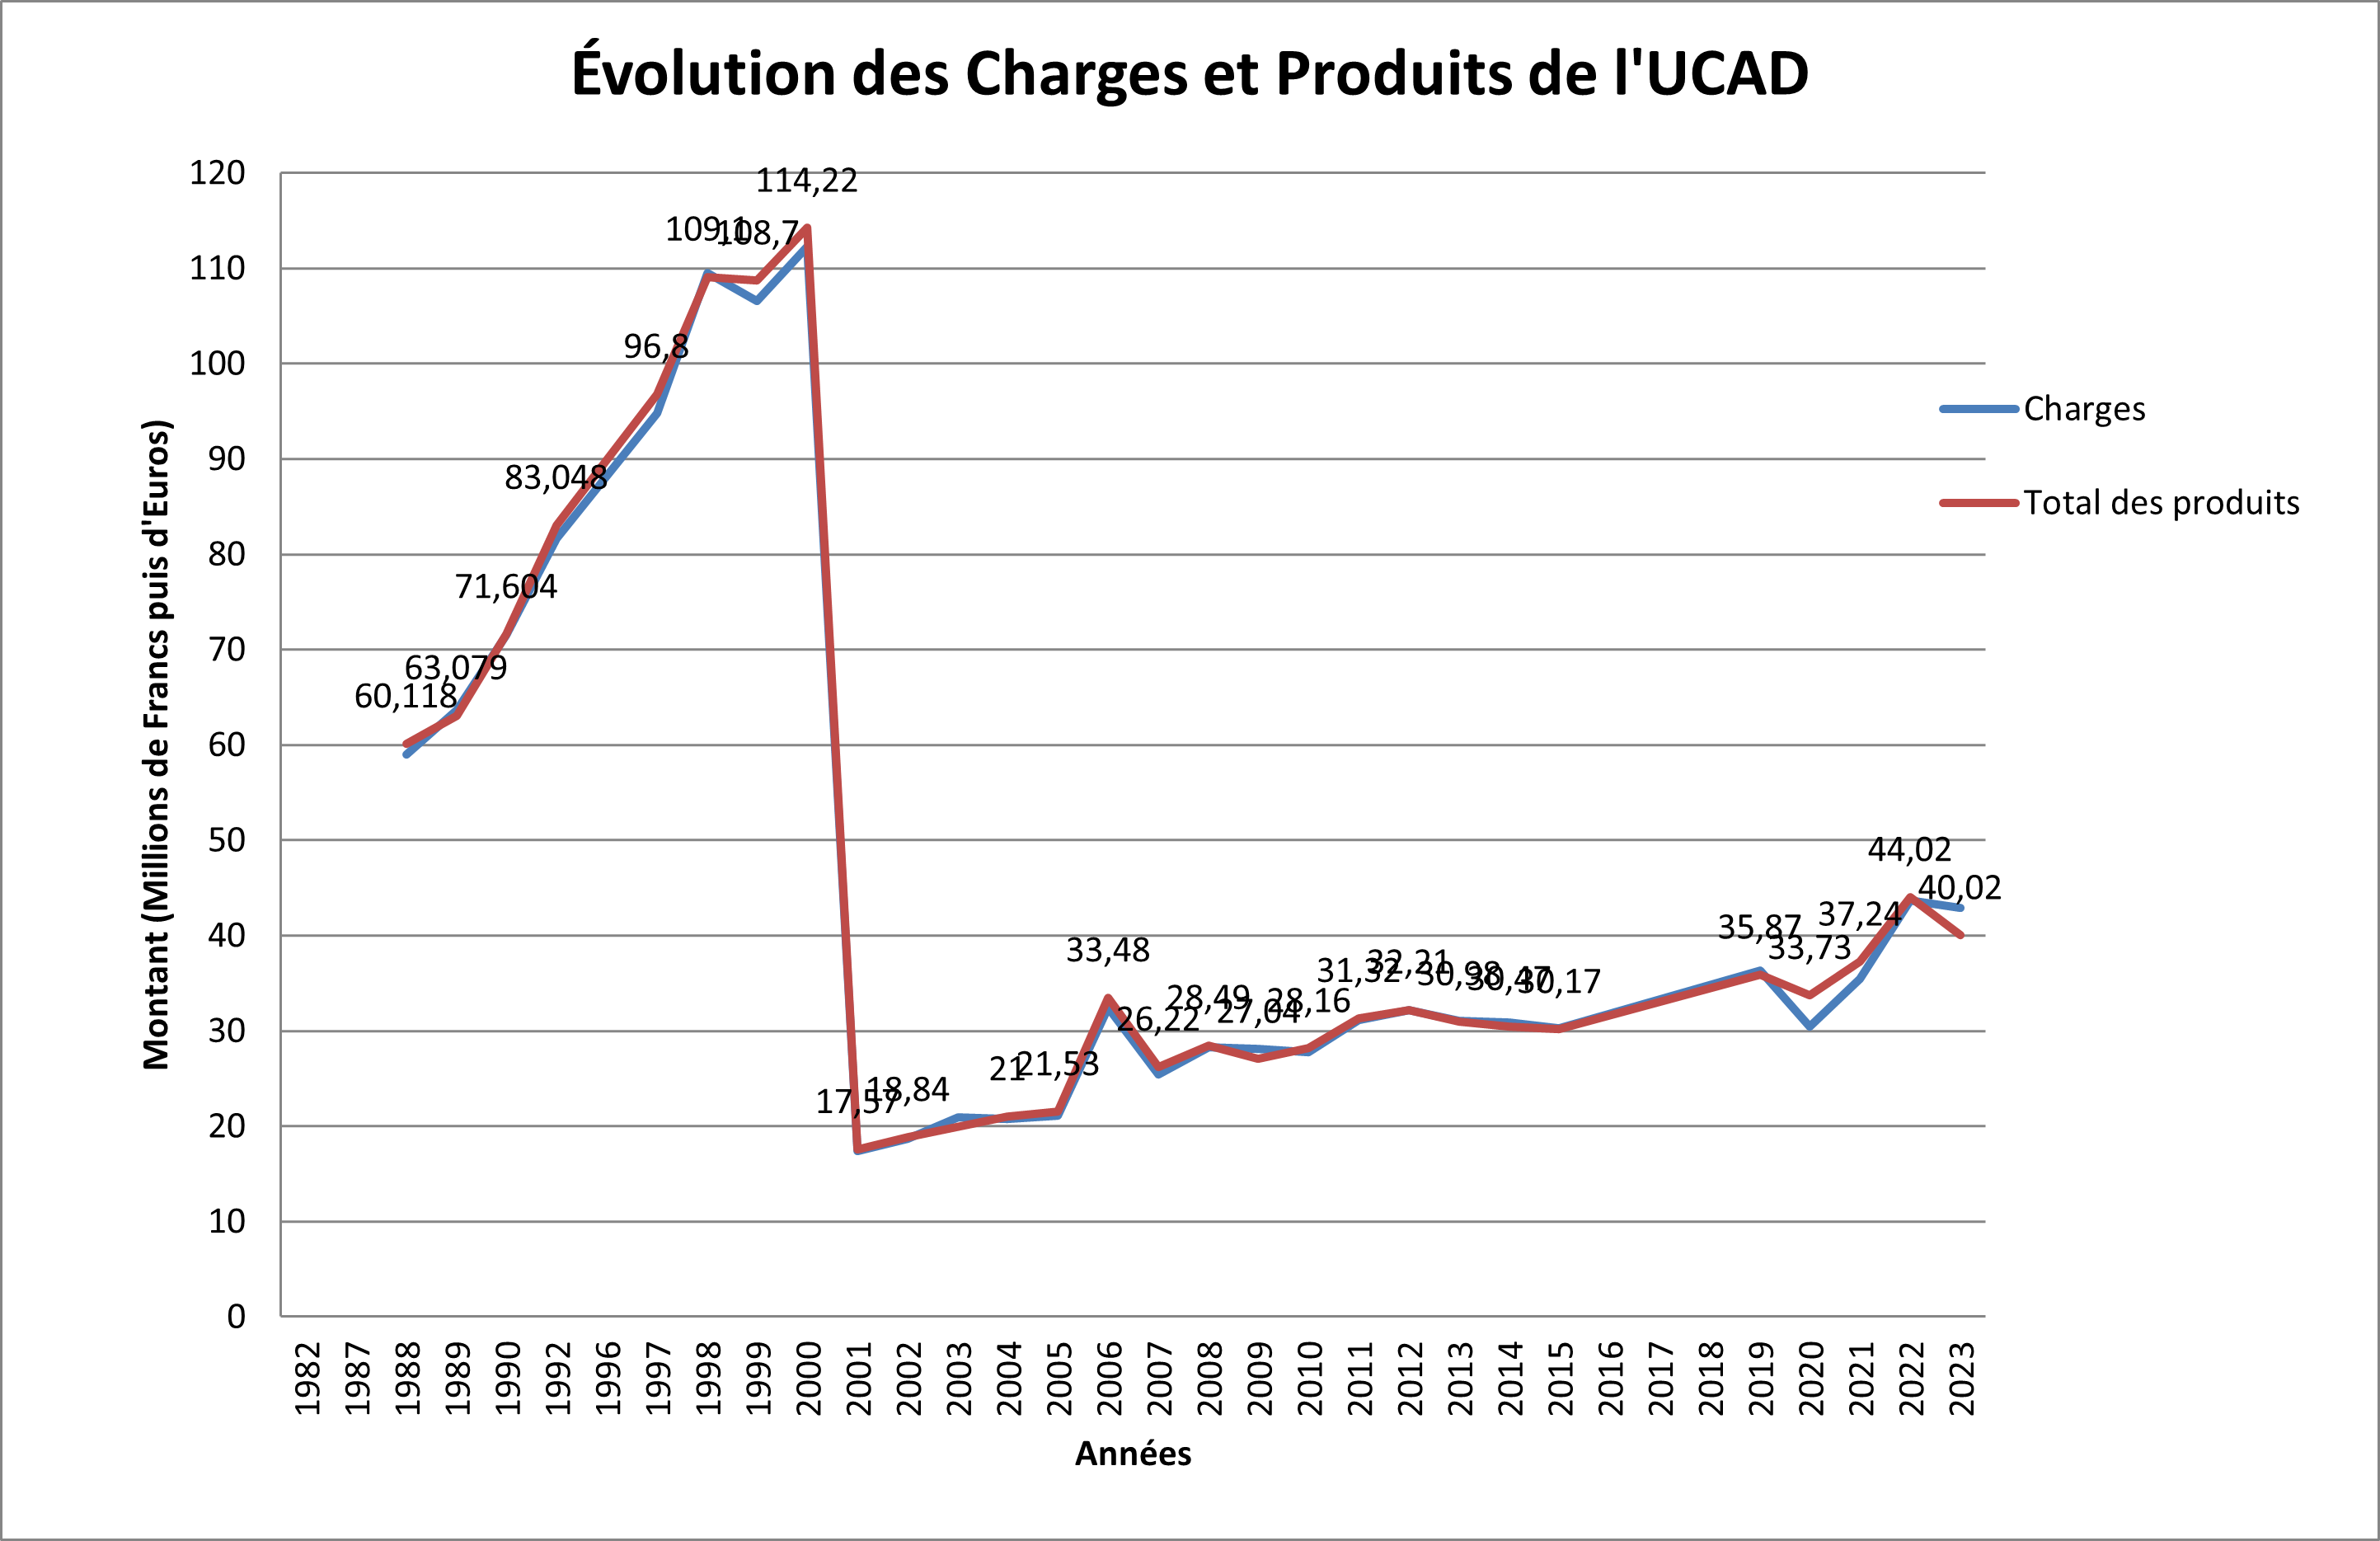
\includegraphics[width=0.75\linewidth]{Illustrations/Image1.png}
    \caption{Évolution des charges et des produits de l'Union entre 1982 et 2023}
    \label{fig:placeholder}
\end{figure}

\begin{figure}[H]
    \centering
    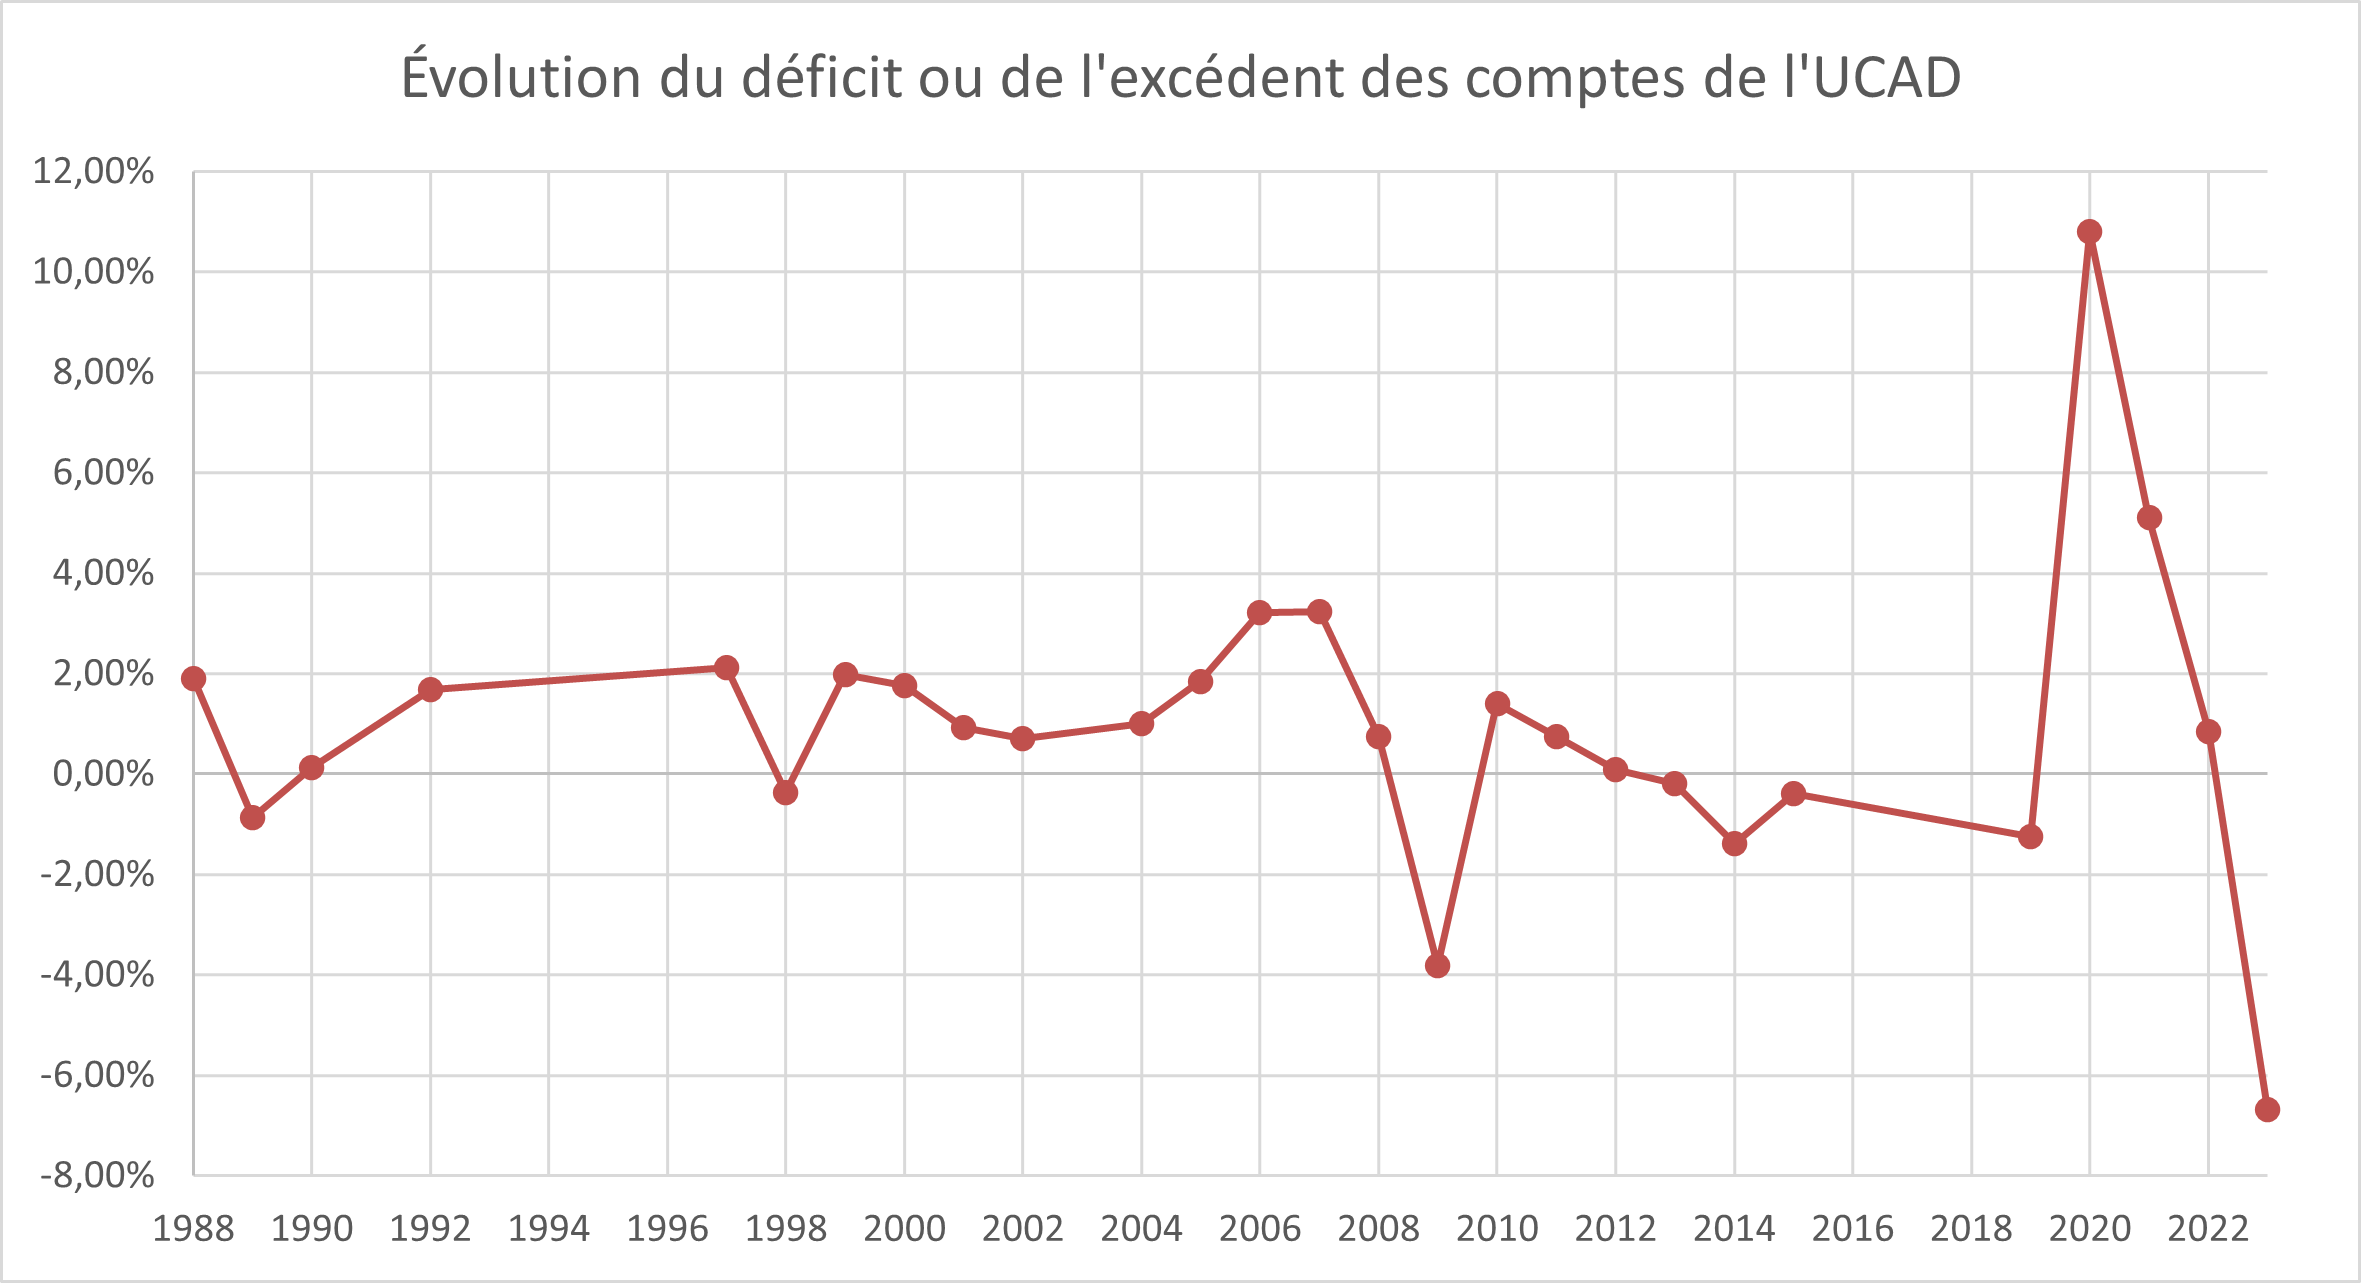
\includegraphics[width=0.75\linewidth]{Illustrations/Image5.png}
    \caption{Évolution du déficit et de l'excédent de l'Union entre 1988 et 2023}
    \label{fig:placeholder}
\end{figure}
\pagebreak

Ce qu'on observe c'est une augmentation croissante des coûts (114,22 millions de Francs étant équivalent à 17,69 millions d'Euros), qui ne se répercute pourtant pas visiblement sur la masse salariale, qui elle reste stable avec une moyenne de 306 employés entre 1982 et 2023\footnote{\cite{noauthor_convertisseur_nodate}}. Le balance entre total des produits et charges est plutôt bonne, avec 7 années enregistrant un déficit, notamment en 2009 des suites de la crise financière. Le large excédent de 2020 s'explique lui par les larges subventions exceptionnelles allouées par l'État au moment du COVID afin de faire face à la pandémie et à la cessation brutale des activités. 

\begin{figure}[H]
    \centering
    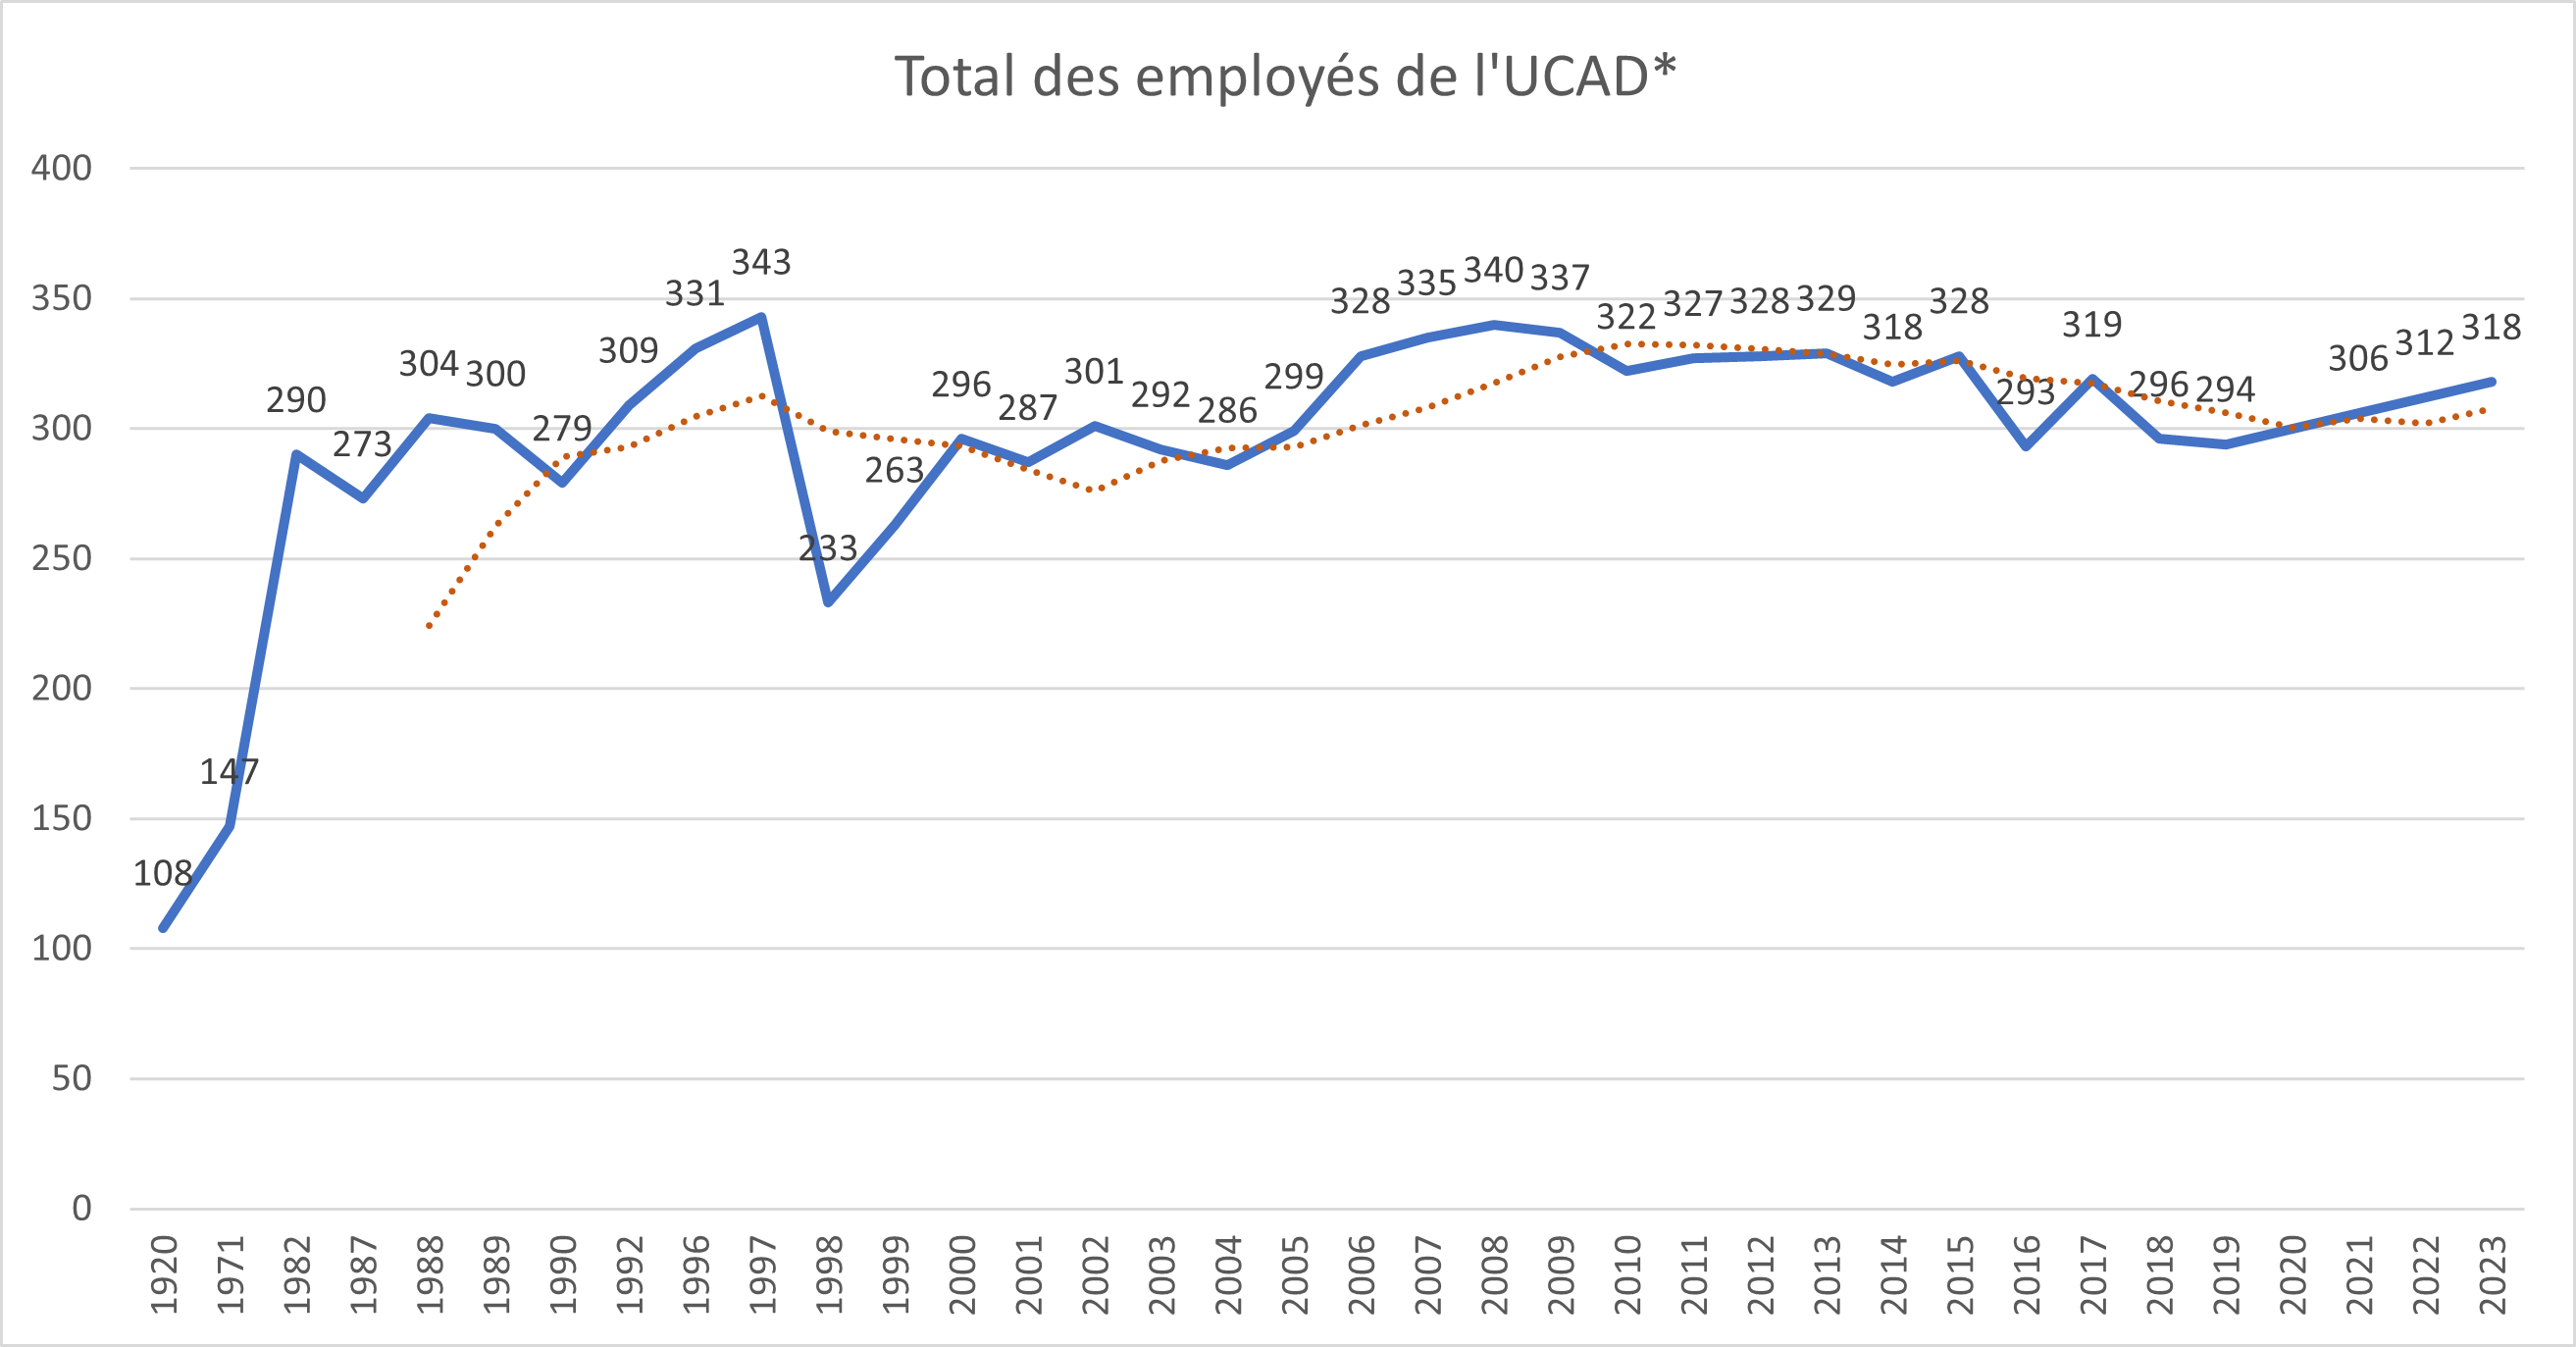
\includegraphics[width=0.75\linewidth]{Illustrations/Image8.png}
    \caption{Évolution du nombre d'employés de l'UCAD}
    \label{fig:placeholder}
\end{figure}

\textit{*Sauf secteurs non-conventionnés (Ateliers du Carrousel et École Camondo).}

Pour le cas qui nous intéresse particulièrement ici nous voulons nous pencher sur l'évolution des ressources humaines au sein du musée des Arts Décoratifs par rapport au reste de l'Union (à l'exclusion des secteurs non-conventionnés). Cela nous permet de quantifier aussi l'importance numérique en terme de répartition des moyens humains, que prend le musée. 

\begin{figure}[H]
    \centering
    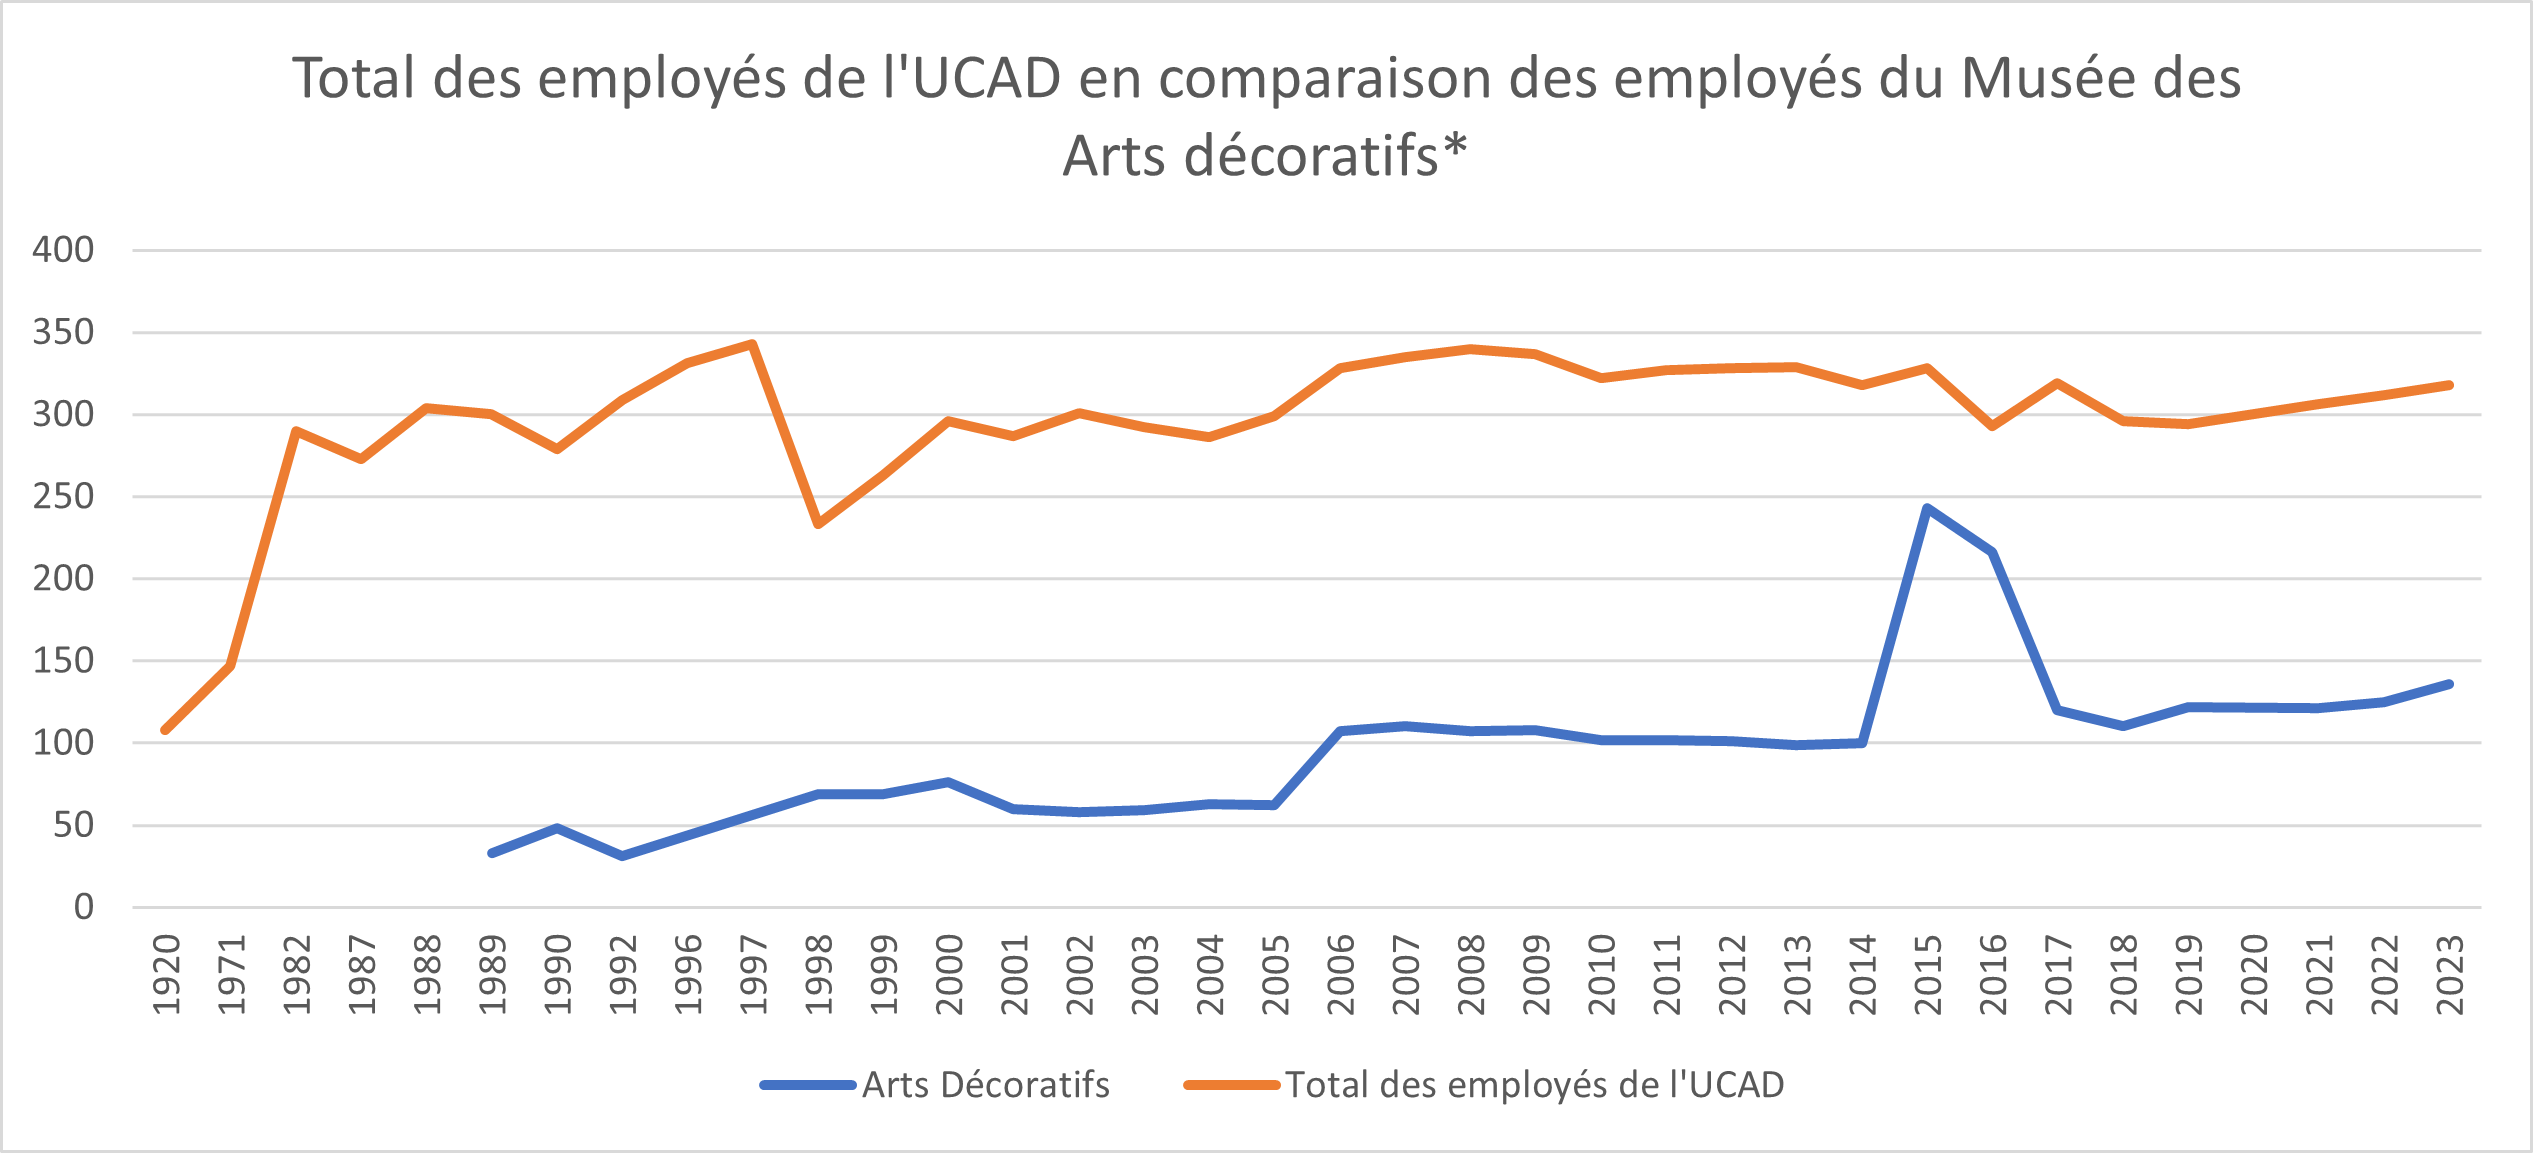
\includegraphics[width=0.75\linewidth]{Illustrations/Image10.png}
    \caption{Évolution des employés du musée des Arts Décoratifs comparé à l'ensemble du personnel entre 1989 et 2023}
    \label{fig:placeholder}
\end{figure}

Ce décompte spécifique pour le musée Arts décoratifs exclut les services techniques et les services communs des musées. Ce qu'on observe c'est que les Arts Décoratifs gagnent peu à peu en importance, notamment entre 2005 et 2006 où on observe presque un doublement des effectifs au musée. Cependant, le pic de 2015 s'explique par la fusion de tous les musées en une seule grande entité, ce qui regroupe tous les employé\wokisme e\wokisme s des musées sous la même appellation \enquote{Direction des musées} dans les sources postérieures. Les tendances à la baisse des années suivantes laissent apparaître une reconfiguration du partage salariale entre les corps de métiers au sein de l'Union, doublé d'une baisse générale de l'effectif entre 2015 et 2016. \hfill \break

\pagebreak

\begin{figure}[H]
    \centering
    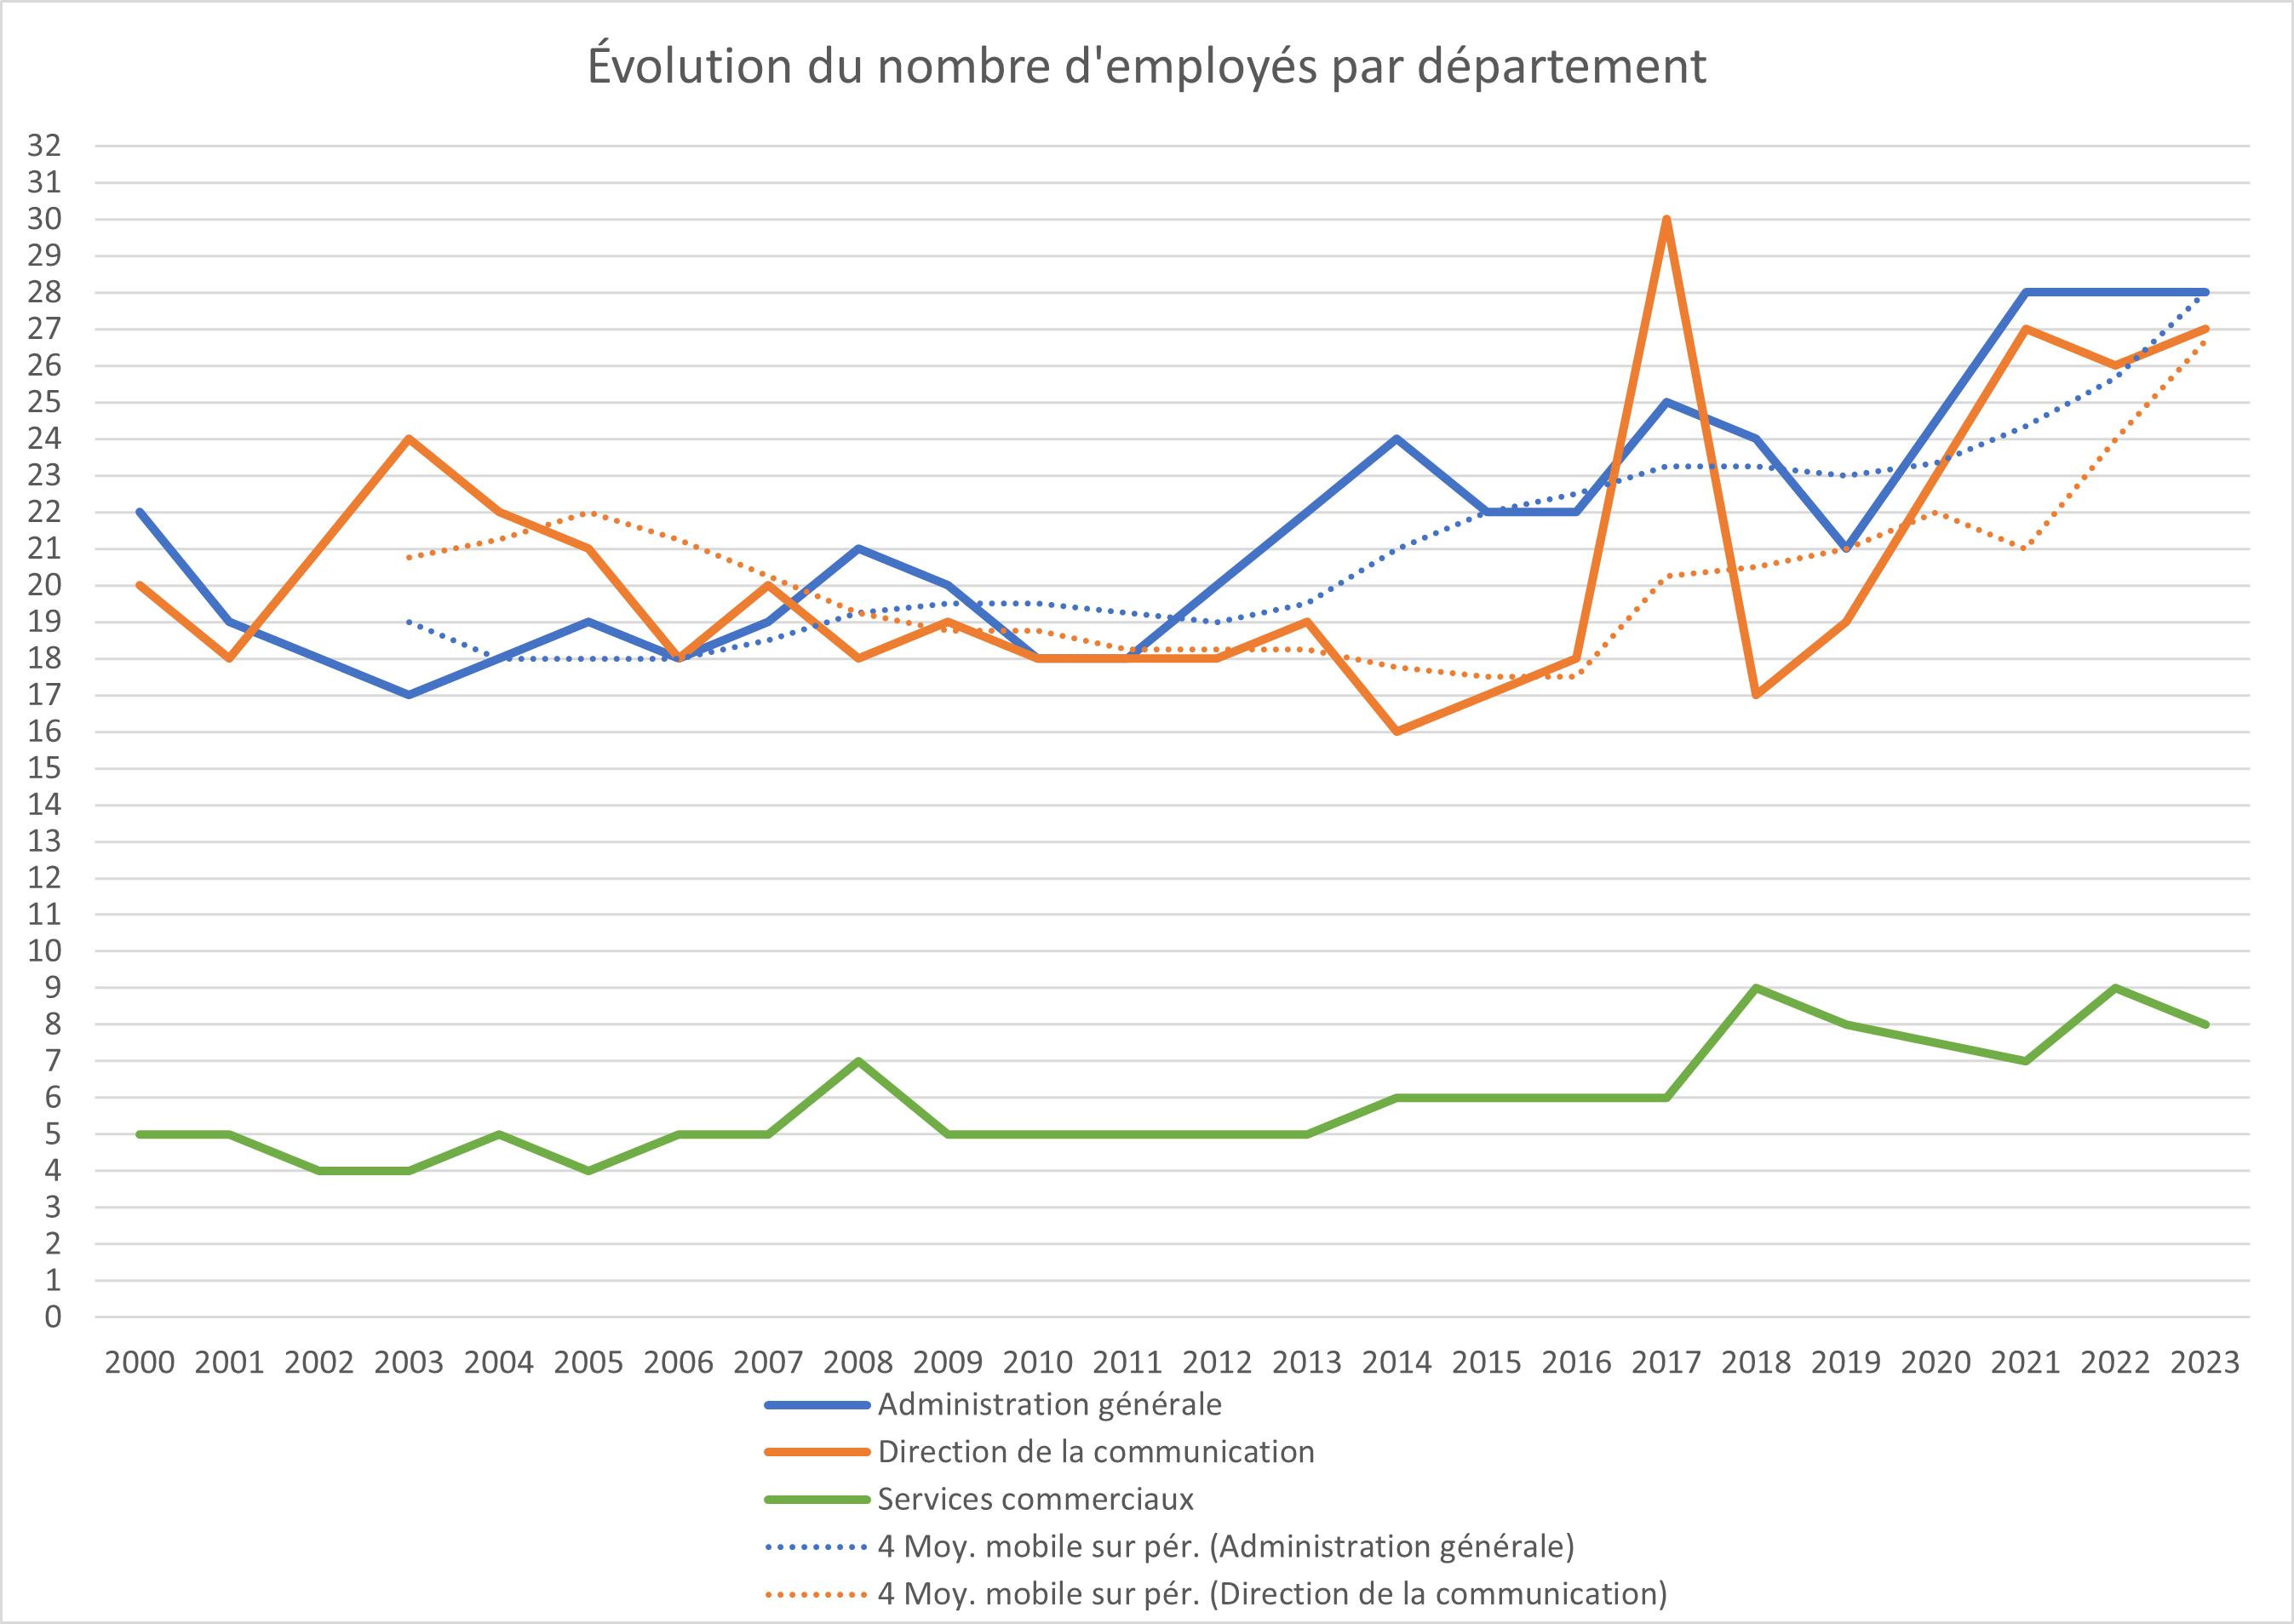
\includegraphics[width=0.75\linewidth]{Illustrations/Image12.png}
    \caption{Évolution du nombre d'employés par départements entre 2000 et 2023}
    \label{fig:placeholder}
\end{figure}

Cette reconfiguration des services du musée s'accompagne d'une tendance d'embauche à la hausse dans les secteurs commerciaux, de la communication et dans la direction. Cependant, ce qui n'apparaît pas ici dans nos visualisations, et qui pourtant est présent dans les rapports d'activités est la répartition entre C.D.I. et C.D.D. au sein de l'Union. Apparaît aussi dans les sources les pourcentages des employé\wokisme e\wokisme s par ancienneté et tranches d'âges, qui pourraient constituer une étude à part entière\footnote{\cite{noauthor__1982}}. Pour ce qui est est de la répartition entre contrats courts et contrats longue durée on observe une augmentation très nette du recours au C.D.D. entre 2010 et 2023 par rapport aux périodes précédentes. Entre 2000 et 2009 on passe de 17 à 27 employé\wokisme e\wokisme s en C.D.D., avec une moyenne autour de 19 sur la période. En 2010, on dénombre 15 employé\wokisme e\wokisme s en C.D.D. contre 51 en 2023, ce qui représente une hausse de 240\% du recours au C.D.D. dans l'Union (à l'exception des secteurs non-conventionnés), avec une moyenne de 35 C.D.D. Du côté des C.D.I., on trouve 302 employé\wokisme e\wokisme s en contrats longue durée en 2010, contre 261 en 2023, soit une baisse de 13,6\%. Si on compare avec la masse salariale totale, les deux années 2010 et 2023 sont plutôt proches avec 322 employé\wokisme e\wokisme s en tout en 2010 et 318 en 2023. 

Ces changements dans la gestion et la précarisation des postes est peut-être à mettre en rapport avec le fait que sur la période concernée (2010-2023), l'Union enregistre 5 des 7 années déficitaires sur ses comptes entre 1988 et 2023. Pourtant quand on observe avec le schéma ci-dessous cela correspond à une période où l'Union se finance en majorité à l'exception des années 2019 à 2022, en gardant bien à l'esprit que cette période correspond aussi à un moment exceptionnel avec les subventions liées au COVID. 

\begin{figure}[H]
    \centering
    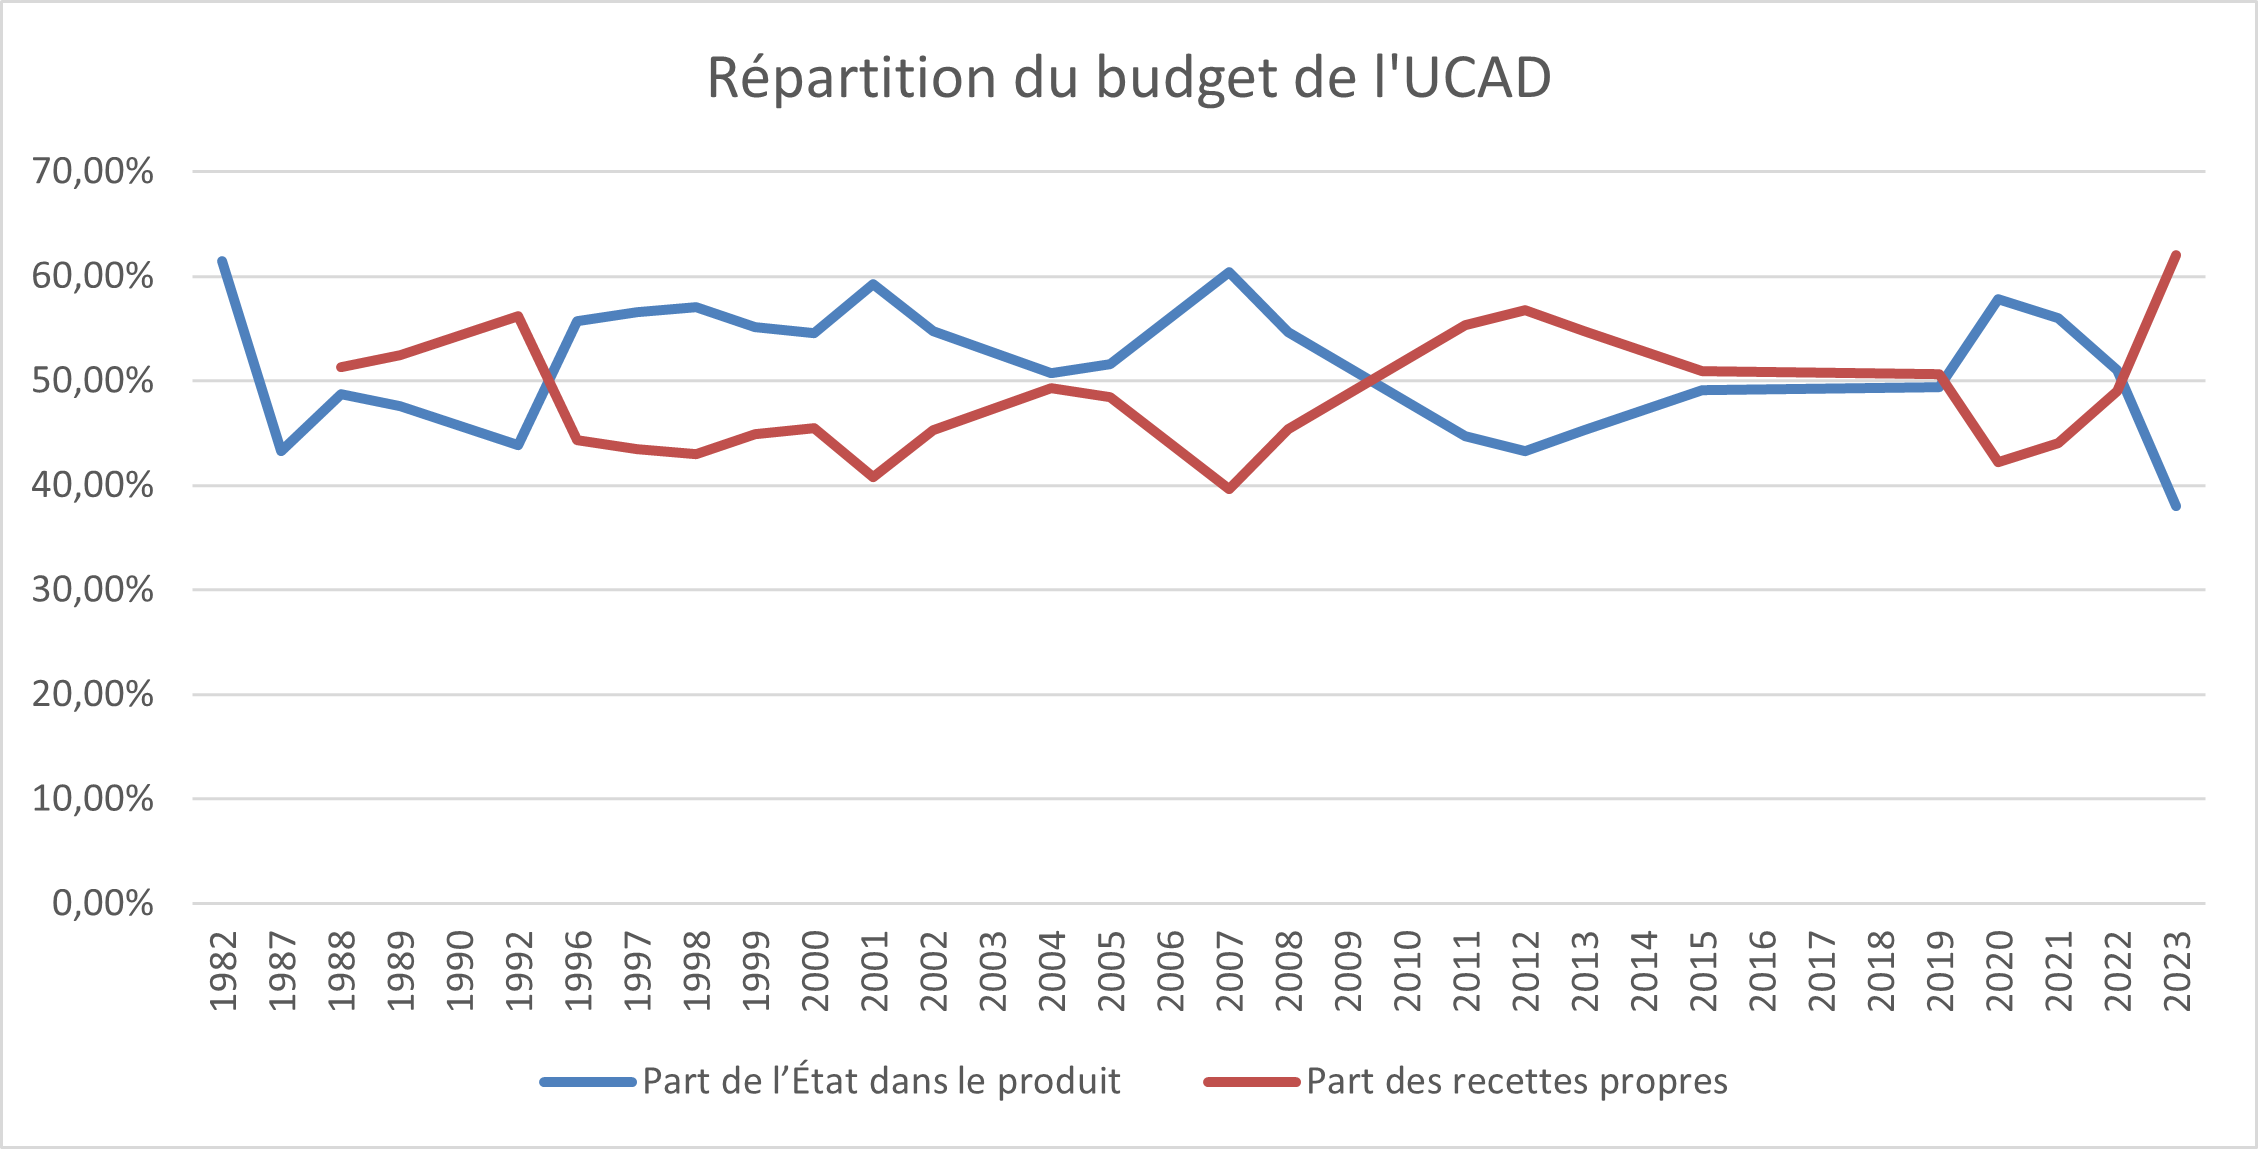
\includegraphics[width=0.75\linewidth]{Illustrations/Image2.png}
    \caption{Évolution de la part de l'État et des revenus propres de l'UCAD dans le total des produits entre 1982 et 2023}
    \label{fig:placeholder}
\end{figure}

\begin{figure}[H]
    \centering
    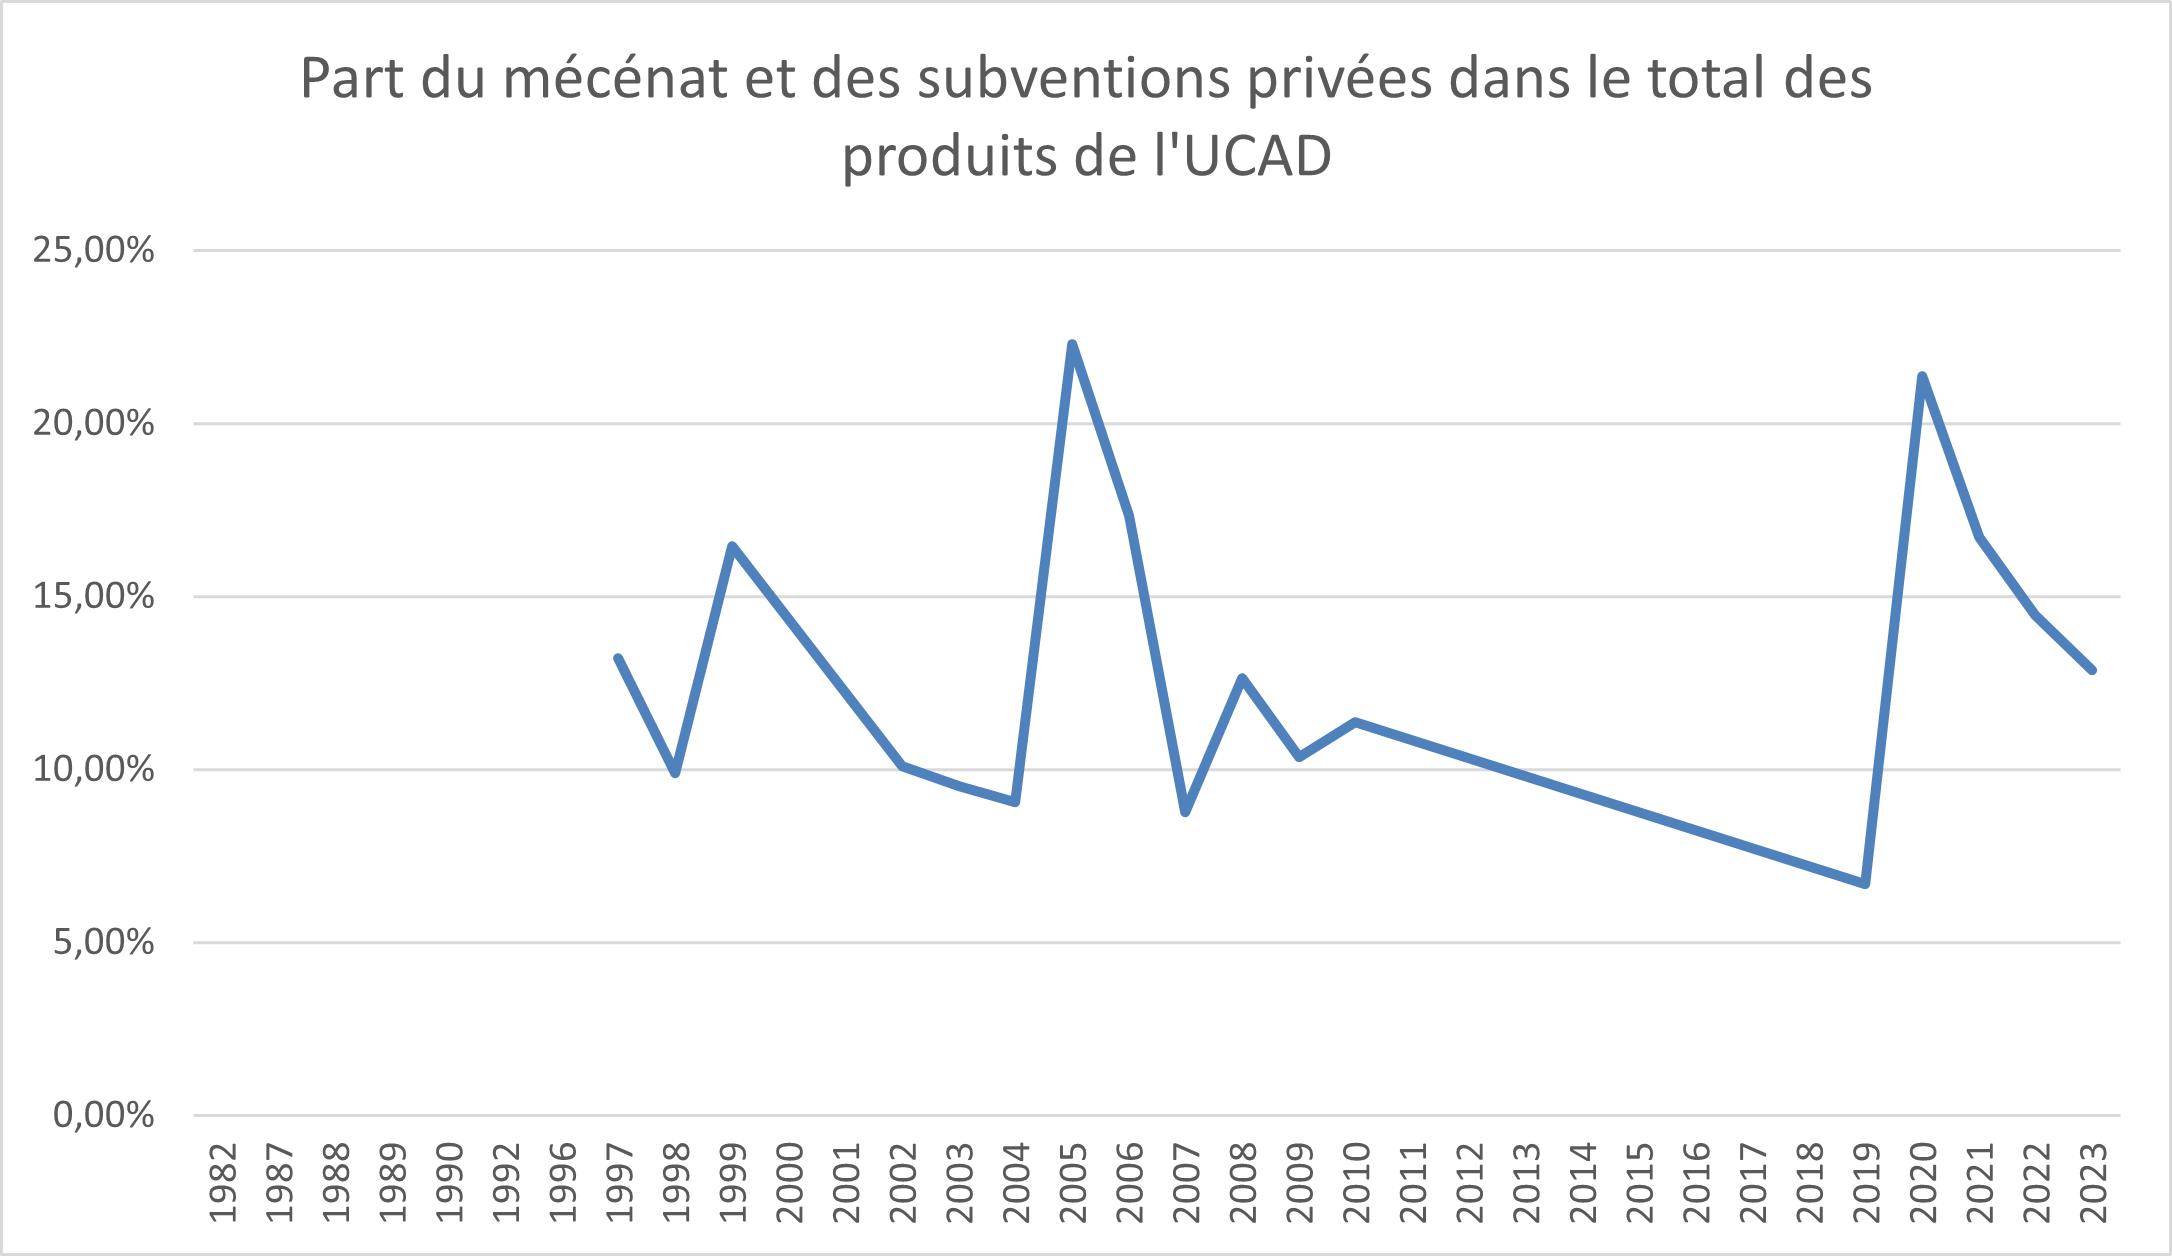
\includegraphics[width=0.75\linewidth]{Illustrations/Image3.png}
    \caption{Évolution en pourcentage de la part du mécénat et des revenus des privatisations sur les recettes propres de l'Union entre 1997 et 2023}
    \label{fig:placeholder}
\end{figure}

Enfin, si on prend en compte cette dernière visualisation, nous pouvons peut-être mettre en rapport cette tendance avec la baisse du mécénat et des revenus issus des privatisations sur la même période. Souvent, les postes liés à des expositions, ou à des chantiers de collections, de restauration ou de réhabilitations, sont des postes mécénés comme le prévoit la convention qui lie l'État à l'UCAD. Aussi, il est bon de souligner qu'en vertu de ladite convention, c'est l'État qui contrôle le plafond d'emploi de l'Union et qui dicte le nombre de postes permanents auxquels l'association peut pourvoir. Les raisons de cette baisse peuvent donc aussi être plus largement politiques et conjoncturelles, au gré des nominations au Ministère de la Culture ou des budgets votés à l'Assemblée, mais pour déterminer cela une étude approfondie serait nécessaire, nous ne pouvons avancer ici que des pistes non vérifiées. 

Pour conclure, nous voulons évoquer un état de fait éloquent posé en 1991 par le Directeur de l'Union d'alors, Antoine Riboud, au cours d'un entretien accordé au Monde. Ce qu'il évoque, après deux années à la tête de l'Union, représente une partie des spécificités structurante de l'UCAD : \enquote{Globalement, le bilan est très positif. L'UCAD regroupe des musées, des écoles qui tous vivent très pauvrement. Le personnel n'a pas le même salaire que celui du Louvre. La conservation est peu nombreuse, dévouée, mais très compartimentée. C'est une entreprise qui a besoin de se moderniser, d'évoluer. Pendant un an, il a fallu s'assurer qu'on restait bien rue de Rivoli. Nous avons, finalement, eu gain de cause}\footnote{\cite{noauthor_entretien_1991}}. Cette citation illustre bien, en effet, le constant danger qui plane au dessus de l'institution, de n'être pas renouvelée au Pavillon de Marsan et dans l'aile Rohan, le manque de moyens structurels en comparaison d'autres institutions patrimoniales publiques et l'aspect pluriel et fragmenté de l'institution. C'est ce dernier aspect, et les évolutions organisationnelles en termes de système d'information et de gouvernance mis en place au musée que nous allons étudier dans la fin du présent chapitre afin de rendre compte, aussi fidèlement que possible de l'état de l'organisation actuelle.

\section{De nouveaux musées et de nouveaux services}

L'histoire des musées qui composent désormais le MAD remonte un peu avant le début de notre période avec l'apparition de deux entités dans l'escarcelle des Arts décoratifs. En 1978 est inauguré le musée de l'affiche\footnote{\cite{siguret_ir_2001}. p. 1.}. Il est basé sur l'ancien fonds d'affiches de la bibliothèque des arts décoratifs, et son domaine d'activité est étendu. Il sera rebaptisé Musée de la publicité et transféré dans l'aile Rohan en 1999. De même le Centre national d'information et de documentation sur les métiers d'art (CNIDMA), est inauguré en 1974 et incorporé au musée des arts décoratifs comme département dès 1990. Pendant notre période, en 1986 est inauguré le Musée des arts de la mode, fruit d'une collaboration entre l'UCAD et l'Union française des arts du costume. Il rouvre ses portes en 1997 sous le nom de musée de la mode et du textile. Toutes ces entités séparées viendront fusionner dans un même musée regroupant toutes les anciennes composantes en 2015. C'est de cette structuration qu'hérite le système d'information actuel. Les données des différentes collections reflètent encore souvent cette répartition dans les bases du musée. Il n'est pas rare de retrouver les noms de ces anciennes institutions en en-tête des dossiers et des classifications. La fusion a eu pour effet de tout regrouper sur un faible nombre de volumes, il existe 2 volumes principaux à l'heure actuelle, qui regroupent l'ensemble des données du musée avant 2020-2021. De cette histoire naturelle des institutions et des enjeux techniques contemporains, sont nées plusieurs problématiques et états de fait qu'il est important de garder à l'esprit dans le cadre de notre étude. L'état des fonds, la dispersion des informations et le système d'information telle qu'il s'est développé sont autant de paramètres à prendre en compte pour le déploiement et la pérennisation de nouvelles méthodes de traitements au sein du musée. 

C'est la raison pour laquelle nous voulons revenir sur l'histoire du déploiement des systèmes informatiques au sein du musée, afin de contextualiser et de remettre en perspective les enjeux passés et présents qui encadrent les collections et leur gestion. Nous allons aussi, dans un second et dernier temps, revenir quelque peu sur l'histoire récente de la bibliothèque et du service d'archives afin de mettre en lumière une autre partie des problèmes qui se posent aujourd'hui aux conservateurs tant des musées et des bibliothèques. 

\subsection{L'informatisation croissante}

Les premières réflexions autour de la nécessité d'informatiser les collections émergent dès le début des années 1990. On en retrouve des traces dans les archives de l'UCAD : \enquote{Les études préalables à l'informatisation des collections sont engagées pour démarrer en 1991}\footnote{\cite{noauthor__1991}. p. 8.}. Le président de l'UCAD évoque aussi ce chantier et la première difficulté qu'il rencontre : le manque de moyens. À la question \enquote{Quel intérêt accordez-vous à la conservation ?}, il répond : \enquote{La première chose à faire, c'est de mettre nos collections sur ordinateur, pour estimer nos richesses. Cette informatisation demandera des moyens importants qui devront figurer dans notre budget de fonctionnement}\footnote{\cite{noauthor_entretien_1991}}. Outre une vision, peut-être partielle des enjeux de conservation, il souligne un point important : être en mesure de pleinement comptabiliser tout ce qui se trouve dans les collections de l'Union. En avril 1996 est lancé la présence de l'UCAD sur internet, la même année on voit la mise en place du premier réseau interne à l'Union qui permet d'accéder aux fiches des œuvres, aux notices de la bibliothèque et, après harmonisation, aux fonds des centres documentaires\footnote{\cite{noauthor__1996}. p. 11 et 13.}. 

Durant les années qui suivent, le parc informatique se développe, les différentes institutions, qui composent l'Union, sont progressivement connectées à internet. Au début des années 2000, un logiciel de gestion de parc informatique est mis en place et les premières campagnes de numérisation massive des albums Maciet ont lieu, pour permettre aux usagers de la bibliothèque de les consulter sur des postes ou sur internet\footnote{\cite{noauthor__1982}. Rapport 2002, p. 54-55.}. Les services informatiques sont aussi sollicités, pendant la première décennie des années 2000, dans divers projets multimédias, de réalisation de documentaire ou de films sur les expositions et leur préparation. En 2010, le SI prépare la mise en ligne des collections. L'année 2020 est une année charnière pour comprendre l'état du système d'information actuel, des documents et des collections du MAD de nos jours. Avec le confinement, et la nécessité de passer en distanciel les activités, le MAD a été massivement basculé sur la suite Microsoft Teams pour continuer ses activités, ce qui a eu pour effet de fragmenter l'information entre des groupes par département et de confier toutes les données du musée à un acteur américain. En plus du coût, l'export vers Teams a eu comme conséquence d'effacer une partie des métadonnées des fichiers au moment de l'import, ce qui pose un certain nombre de problèmes actuellement, notamment pour le service d'archives. 

L'autre grand changement cette année-là est la reprise du chantier \enquote{de changement du système de gestion et de publication des collections et des archives du musée}\footnote{\cite{noauthor__1982}. Rapport d'activités 2020, p. 68.}. Ce travail a donné lieu à une définition de l'architecture cible et à un état des lieux des médias. C'est ce travail qui a amené à la mise en place d'un contrat avec Skinsoft pour la mise en place de la base Arcadie, qui ne sera mise en production qu'en 2022.

Pendant toute l'histoire récente de l'Union, l'informatisation croissante des activités, et la mise en place d'un Service Informatique a progressivement accompagné le développement de l'institution. De la mise en place des premiers postes informatiques, au déploiements de solutions extérieures pour la gestion RH par exemple, en passant par les premières numérisations, le branchement à Internet et les projets multimédias, le SI n'a pas toujours servi le même rôle. Aujourd'hui il est principalement en charge du parc informatique et technologique du MAD, il gère son intranet, les quelques serveurs qui sont encore en interne, sa billetterie, sa sécurité informatique et se charge de l'implémentation de solutions clef en main de type \textit{Software as a Service} pour les services du musée\footnote{\textit{cf}. le \textbf{\hyperref[sec:Glossaire]{Glossaire}} pour le terme \enquote{\textit{Software as a Service}}, p.~\pageref{sec:Glossaire}.}. 

\subsection{La création des archives et l'évolution de la bibliothèque}

Afin de parler de la création d'un des derniers services de l'Union, le service des archives, nous devons revenir brièvement sur l'histoire récente de la bibliothèque, d'où provient l'initiative des missions archivistiques au sein de l'association, bien avant la création officielle du service en 2014. Depuis la fin du \textsc{xx}\textsuperscript{e}~siècle la bibliothèque connaît un lent déclin de ses fréquentations et une érosion de ses collections au profit du musée. Autrefois, cœur vibrant de l'UCAD, la bibliothèque connaît une chute vertigineuse de sa fréquentation. Alors qu'elle a plus de 25 000 visiteurs par an en 1955\footnote{\cite{noauthor__1955}. p. 6.}, avec un pic à 30 000 visiteurs en 1964\footnote{\cite{noauthor__1965}. p. 10.}, elle enregistre 24 360 visiteurs en 1988\footnote{\cite{noauthor__1982}. Rapport d'activités 1988.}, puis seulement 5000 en 2024\footnote{Donnée récoltée auprès des personnels de la bibliothèque en juillet 2025.}. L'informatisation croissante est un facteur évident, du fait de l'accessibilité accrue des ressources en ligne, et des campagnes de numérisations. Cependant d'autres facteurs peuvent aussi être pris en compte. 

Alors qu'en 1996 les documents d'archives du \enquote{Plan stratégique de l'UCAD} mentionnent la volonté de faire de l'UCAD un centre de la recherche sur les arts décoratifs\footnote{\cite{noauthor__1996}. p. 12.}. L'érosion successive des fréquentations et l'abandon progressif de plusieurs initiatives pour la recherche, comme le carnet Hypothèses \enquote{Du Beau dans l'utile}, couplés avec la rétrogradation récente de la direction de la bibliothèque en simple service, marque un climat de déclin pour la bibliothèque et sa mission de recherche\footnote{\cite{rivoire_du_2021}}. 

Pour ce qui est des archives, la première formalisation moderne d'un outil pour la mise en place d'une démarche proprement archivistique au sein de l'Union se cristallise autour de l'Instrument de Recherche produit en 2001 par Florence Siguret. Cependant, ce dernier mentionne une initiative antérieure lancée en 1977 par Yolande Amic, conservateur du musée des Arts décoratifs à ce moment-là. Il faut rappeler qu'en dépit de l'ancienneté de l'association, jusque-là \enquote{ces archives ont été stockées sans classement ni inventaire au fil des ans, [...] ont subi plusieurs déménagements [pour enfin] être déménagées au sein de la bibliothèque des arts décoratifs, non sans dommages}\footnote{\cite{siguret_ir_2001}. p. 2.}. À ces péripéties s'ajoutent les consultations \enquote{plus ou moins scrupuleuses} des chercheurs, la mauvaise ré-intégration ou la perte de certains documents et le fait que certains services conservent encore leur propres archives, et l'on obtient des fonds obligatoirement lacunaires. 

Ce dernier point illustre bien une des tensions au sein du MAD qui persiste encore à l'heure d'aujourd'hui. En effet, l'association, relevant du droit privé mais ayant à sa charge des collections publiques, produit de fait des archives publiques. Cependant, du fait de son histoire elle gère aussi un grand volume d'archives privées de particuliers et de collectionneurs, mais \enquote{la trop forte interpénétration entre archives publiques et archives privées rend caduque une quelconque délimitation}\footnote{\cite{siguret_ir_2001}. p. 4.}. Pour la mission de l'archiviste il peut, de ce fait, devenir compliqué d'accéder, de centraliser et de pouvoir traiter certains dossiers de services ou de personnes quand ces dernières ne perçoivent pas ce qu'ils produisent dans le cadre de leur activités comme des archives publiques. Enfin, le dernier point de tension, qui joue un rôle important pour nous dans notre compréhension de l'état des collections en vue de leurs traitements, est la confusion ou requalification d'un objet comme œuvre d'art. Nombreux fonds ont été déplacés de la bibliothèque aux collections du musée lorsque certain\wokisme e\wokisme s se sont rendus compte de la valeur esthétique qu'ils pouvaient avoir. Ce point pose, par ailleurs, problème dans les relations entre les services. 

C'est vers 2013-2014 que Carole Pilarz, bibliothécaire adjointe se forme et assume brièvement des fonctions d'archiviste pendant que Nathalie Baueur établissait un état des lieux en vue de l'embauche d'Élise Barzun en 2014 et de la création officielle du service d'archives\footnote{Propos recueillis auprès de Karine Bomel, Responsable du pôle archives de la bibliothèque des arts décoratifs, le 22/08/2025.}. Puis, en 2017 lorsque la réflexion sur la mise en place d'un nouvel outil de gestion des collections émerge, réflexion qui aboutira au contrat avec Skinsoft et au déploiement d'Arcadie en 2022, les équipes du musée intègrent d'emblée la dimension archivistique dans le cahier des charges du nouvel outil. Ce dernier devant pouvoir permettre de gérer les fiches des œuvres, et ce qui a été plus tard regroupé sous le terme de \enquote{ressources documentaires}, afin de documenter au mieux les œuvres et leur histoire.

\chapter*{Conclusion}

Nous avons parcouru au pas de charge plus d'un siècle et demi d'histoire afin de donner aux lecteurs\wokisme trices un bref aperçu, aussi fidèle que possible, du caractère unique de l'institution que nous étudions et de son souffle si particulier. De laboratoire d'enseignement pour les arts décoratifs ouvert à tous, à institution patrimoniale ayant à sa charge des collections publiques dans l'aile d'un des plus beau palais du monde, en passant par association de passionnés et de généreux esthètes en quête de toit, l'Union Centrale des Arts Décoratifs surprend par sa forme et son caractère si particulier dans le paysage muséal français. C'est bien dans son développement si unique que nous devons comprendre les enjeux qui l'animent aujourd'hui, enjeux qui déterminent en grand partie la nature des projets que nous pouvons y développer. Que ce soit les volontés d'informatisation précoce des collections, la place des différents musées, celle de la bibliothèque, la création récente du service des archives, ou bien le basculement au tout numérique en raison de la pandémie de Covid-19. Tous ces développements organiques d'une association polycéphale dictent la compréhension que nous devons avoir de l'état de ses collections et donc de la manière dont nous pouvons tenter d'en proposer un traitement automatisé. C'est la raison pour laquelle, dans le second mouvement de ce travail, nous nous attachons à décrire l'environnement de recherche dans lequel se situe le projet TORNE-H, les réalisations techniques du stage et les premiers résultats de l'introduction de l'IA au musée.